%%%%%%%%%%%%%%%%%%%%%%%%%%%%%%%%%%%%%%%%%%%%%%%%%%%%%%%%%%%%%%%%%%%%%%%%%%%%%%%%%%%%%%%%%%%%%%%%%%%%%
% This template is distributed with ABSOLUTELY NO WARRANTY.
% It serves as a guideline and constitutes a basic structure for a
% thesis/dissertation. The user assumes full responsibility for formatting
% and typesetting their document and for verifying that all the thesis
% requirements set by the University of Tennessee are met. Please refer to the most
% recent UT thesis guide (http://web.utk.edu/~thesis/thesisresources.shtml)
% or contact the thesis consultant (http://web.utk.edu/~thesis/).
% Please report any bugs to the thesis consultant.
%%%%%%%%%%%%%%%%%%%%%%%%%%%%%%%%%%%%%%%%%%%%%%%%%%%%%%%%%%%%%%%%%%%%%%%%%%%%%%%%%%%%%%%%%%%%%%%%%%%%%
% O P T I O N S:
% 1. thesis/dissertation
% 2. monochrome
% 3. all options provided by the report class
\documentclass[thesis,letterpaper,12pt]{utthesis} % thesis, one side
% some alternatives are:
%\documentclass[thesis,monochrome,letterpaper,12pt]{utthesis} %thesis, one side, monochrome text
%\documentclass[thesis,twoside,letterpaper,12pt]{utthesis} % thesis, two side
%\documentclass[thesis,monochrome,twoside,letterpaper,12pt]{utthesis} % thesis, two side, monochrome text
% for a dissertation, replace the thesis option by dissertation:
% \documentclass[dissertation,letterpaper,12pt]{utthesis} . . .
\renewcommand{\baselinestretch}{1.5} 	 % line Spacing
%%%%%%%%%%%%%%%%%%%%%%%%%%%%%%%%%%%%%%%%%%%%%%%%%%%%%%%%%%%%%%%%%%%%%%%%%%%%%%%%%%%%%%%%%%%%%%%%%%%%%
% TO DO: FILL IN YOUR INFORMATION BELOW - READ THIS SECTION CAREFULLY
%%%%%%%%%%%%%%%%%%%%%%%%%%%%%%%%%%%%%%%%%%%%%%%%%%%%%%%%%%%%%%%%%%%%%%%%%%%%%%%%%%%%%%%%%%%%%%%%%%%%%
\title{My Thesis or Dissertation Title}	       % title of thesis/dissertation
\author{My Name}                % author's name
\copyrightYear{2012}            % copyright year of your thesis/dissertation
\graduationMonth{May}           % month of graduation of your thesis/dissertation
\majorProfessor{My Advisor}	    % advisor's name
\keywords{List, Of, Keywords}	% keywords (optional) separated by commas - these are used in the PDF file properties
\viceProvost{Carolyn R. Hodges} % vice provost name
\major{Mechanical Engineering}	% major: Mechanical Engineering, Aerospace Engineering, Mathematics...
\degree{Master of Science}	    % degree: Doctor of Philosophy, Master of Science, Master of Engineering...
\college{Engineering}           % college
\dept{Mechanical, Aerospace and Biomedical Engineering}	% department
\university{The University  of Tennessee, Knoxville}	% school name
% THIS TEMPLATE ACCOMMODATES UP TO 5 COMMITTEE MEMBERS - ENTER ONLY THE NAMES OF THE MEMBERS ON YOUR COMMITTEE
\numberOfCommitteeMembers{2} % enter the number of committee members
\committeeMemberA {Committee Member 1}	% name of first committee member
\committeeMemberB {Committee Member 2}	% name of second committee member
\committeeMemberC {Committee Member 3}	% ... you get the trend!
\committeeMemberD {Committee Member 4}	% if your committee has less than 4 members, you do not need to edit the
\committeeMemberE {Committee Member 5}  % rest of committee names
%%%%%%%%%%%%%%%%%%%%%%%%%%%%%%%%%%%%%%%%%%%%%%%%%%%%%%%%%%%%%%%%%%%%%%%%%%%%%%%%%%%%%%%%%%%%%%%%%%%%%
% LOAD SOME USEFUL PACKAGES
%%%%%%%%%%%%%%%%%%%%%%%%%%%%%%%%%%%%%%%%%%%%%%%%%%%%%%%%%%%%%%%%%%%%%%%%%%%%%%%%%%%%%%%%%%%%%%%%%%%%%
\usepackage{nomencl}                    % produces a nomenclature
\usepackage{float}                      % figure floats
\usepackage{natbib}                     % this package allows you to link your references
\usepackage{graphicx}					% graphics package
\graphicspath{ {figures/}{figures/eps/}{figures/pdf/} }% specify the path where figures are located
\usepackage{fancyhdr}                   % fancy headers and footers
\usepackage{url}                        % nicely format url breaks
\usepackage[inactive]{srcltx}		 	% necessary to use forward and inverse searching in DVI
\usepackage{relsize}                    % font sizing hierarchy
\usepackage{booktabs}                   % professional looking tables
\usepackage[config, labelfont={bf}]{caption,subfig} % nice sub figures
\usepackage{mathrsfs}                   % additional math scripts
%%% PACKAGES THAT ARE PRELOADED WITH THE CLASS ARE: amsmath,amsthm,amssymb,setspace,geometry,hyperref,and color
%%%%%%%%%%%%%%%%%%%%%%%%%%%%%%%%%%%%%%%%%%%%%%%%%%%%%%%%%%%%%%%%%%%%%%%%%%%%%%%%%%%%%%%%%%%%%%%%%%%%%
\begin{document}
    \pagenumbering{alph} % this is needed to clear certain issues with the hyperref package
    %
    \makeApprovalPage % make the approval page - this is the page that needs to be signed & returned to the thesis/dissertation consultant
    \makeETDApprovalPage % make the Electronic Thesis & Dissertation page - this page is kept with the electronic copy
    %
    \addToPDFBookmarks{0}{Front Matter}{rootNode} % create a root node named "Front Matter" in the pdf bookmarks
    \addToPDFBookmarks{1}{Title}{a} % add a pdf bookmark to the title page
    \makeTitlePage % make the title page. Make sure you properly set the \docType
    %
    \pagenumbering{roman}
    \setcounter{page}{2}
    %
    \makeCopyrightPage % make the copyright page
    %
    \addToPDFBookmarks{1}{Dedication}{b} % add a pdf bookmark to the dedication page
    \include{front-matter/dedication} % include the dedication
    %
    \addToPDFBookmarks{1}{Acknowledgements}{c} % add a pdf bookmark to the acknowledgements page
    \include{front-matter/acknowledgements} % include the acknowledgements
    %
    \addToPDFBookmarks{1}{Quote}{d} % add a pdf bookmark to the quotation page
    \include{front-matter/quote} % include a quote
    %
    \addToPDFBookmarks{1}{Abstract}{e} % add a pdf bookmark to the abstract page
    \include{front-matter/abstract} % your abstract
    %
    \addToPDFBookmarks{0}{Table of Contents}{f}
    \tableofcontents % generate a table of contents
    %
    \addToTOC{List of Tables} % this will add the list of tables to the Table of Contents (TOC)
    \listoftables % generate a list of tables
    %
    \addToTOC{List of Figures} % this will add the list of figures to the Table of Contents (TOC)
    \listoffigures % generate a list of figures
    %
    \makenomenclature % OPTIONAL
    \addToPDFBookmarks{0}{Nomenclature}{g} % OPTIONAL
    \printnomenclature[1.25in] % OPTIONAL
    %
    \newpage
    \pagenumbering{arabic}
    \setcounter{page}{1}
    %%%%%%%%%%%%%%%%%%%%%%%%%%%%%%%%%%%%%%%%%%%%%%%%%%%%%%%%%%%%%%%%%%%%%%%%%%%%%%%%%%%%%%%%%%%%%%%%%%%%%
    % INCLUDE THE CHAPTERS STARTING WITH THE NOMENCLATURE IF PRESENT
    %%%%%%%%%%%%%%%%%%%%%%%%%%%%%%%%%%%%%%%%%%%%%%%%%%%%%%%%%%%%%%%%%%%%%%%%%%%%%%%%%%%%%%%%%%%%%%%%%%%%%
    \include{front-matter/nomenclature} % OPTIONAL
    \chapter{Introduction} \label{ch:introduction}
\section{Problem Statement}
Employee turnover has drawn management researchers and practitioners attentions for decades, because employee turnover cost impacts both the operational capabilities and the budget of an organization. Employee turnover is both costly and disruptive to the functioning of most organizations \citep{kacmar2006, mueller1989,staw1980}, and both private firms and governments spend billions of dollars every year managing the issue according to Leonard \citeyearpar{leonard2001}. %check reference
Employee turnover is an employee leaving his current working organization due to variety reasons, such as voluntary quitting, retirement, disability, or death.
The turnover cost involves recruiting, selecting, training and developing \citep{mobley1982, staw1980}. According to the estimation from U.S. Department of Labor, turnover costs a company one third of a new hire's annual salary to % check this sentence
replace an employee, which is about \$500 to \$1500 per person for fast-food industry and \$3000 to \$5000 per person for trucking industry \citep{white1995}. 

Furthermore, turnover also disrupts the social and communication structures, and causes the productivity loss due to the replacement \citep{mobley1982}. Beyond the replacement cost and operational disruption, turnover demoralizes the attitudes of remaining employees and leads to additional turnover \citep{staw1980}. \citet{sagie2002} found that 2.8 million US dollars or 16.5\% of the before-tax annual income was lost for a high tech firm due to the withdrawal behaviors and they concluded that turnover reduced the profit, increased the total risk of organizations, and triggered more turnover for the other employees in the organization. Therefore, understanding and forecasting turnover at firm and departmental levels is essential for reducing it \citep{kacmar2006} and for effective planning, budgeting, and recruiting in the human resource field. 

Many studies have proved that employee turnover has significant effects on organizational performance. \citet{staw1980} summarized the previous studies that turnover reduced the team or work performance and financial performance of organizations, and significantly changed the direction of an organization when top executives leaves. \citet{glebbeek2004} found that overly high employee turnover was harmful for firm performance (profits). According to \citet{hancock2013}'s study, turnover has strong negative relationship with organizational performance in manufacturing and transportation industries. 
According to \citet{kacmar2006}'s study employee turnover caused customer waiting time increasing and reduced the store profits. Turnover also reduces the restaurant profitability and customer satisfaction due to counter productivity declining \citep{detert2007}. On the other hand, the lower turnover rate increase the sales \citep{batt2002}. Overall, unable to predict employee turnover and to replace that individual reduce organizational performance and profits and disrupt the organizational structure. 

Employee turnover prediction help reduce the hiring lead time, and as a results of eliminating the some turnover costs. The lead time of employee turnover and replacement includes six stages, such as, notice, approval, advertisement, interview, background check, and on-board training. An employee usually provides a leaving notice at lease two weeks before the actual leaving date; the employee's manager has approval it and prepare for advertisement and hiring committees (one week); the hiring committees needs two to eight weeks, sometimes even longer, to release the hiring advertisement and select interview candidates; the interview period takes hiring committees one to two weeks to make a final decision; the finalist needs one week to six months background security check; after background check, the employee's on-board and training takes at lease one week to six months. Clearly, a organization usually spends at least two months to replace a new employee. For some governmental organization, the hiring lead time is much longer since their security check takes from three months to six months. Employee turnover forecasting shorten the hiring lead time. The forecasting system provides the predicted turnover number in a year ahead. The HR department determines a final demand number through considering this number and its budget. Regardless employees' notice and approval periods, it can release its advertisement and start to hire immediately based on the final demand or right after receiving a leaving notice. Therefore, understanding and forecasting turnover at firm and departmental levels is essential for reducing it \citep{kacmar2006} and for effective functional lean management system. 
\section{Purpose of study}
The studied governmental organizations have a very long lead time to hiring a new employee, due to the long background security check usually more than 6 months. This study developed a methodology to forecast employee turnover in organizational level to shorten employee hiring lead time. It also investigates turnover seasonal patterns and factors, such as employee demographic information, job categories, and orientations structures, identifies influential financial indexes, measures the magnitude of retention and Early Retirement Incentive program \citep{ERIP} released by (HR) department, forecasts employees's turnover by two causes, retirement and voluntary quitting. The study also simulates the turnover datasets to measure two data biases and examine the forecasting capability of the forecasting models.   
\section{Approach}
Employee turnover forecasting effectively assists the operation of lean management system. Actually, it is crucial part of lean management system \citep{allway2002}. Lean management system, also called toyota production system, is about operating the most efficient and effective organization possible, with the least cost and {\it zero} wastes \citep{jackson1996}. \citet{allway2002} claimed that the employee turnover is significant factors for lean tools. The waste is non-valued-added activities. The high employee turnover are one kind of wastes \citep{kilpatrick2003}. 

Employee turnover forecasting system reduce the wastes causing by the high turnover. It identifies the factors of employee turnovers. The influential factors assists HR to determine specific retention strategies focusing on target employee groups to reduce the turnover rates. According to \citet{yeung1997} and \citet{kochan1992}, "high-commitment" human recourse polices successes the lean management system.   

Further more, Employee turnover forecasting system reduce the setup time of the organization lean management system. \citet{lin1999} claimed that employee turnover leads to lean organization take much more time and far more resources to select and train a new employee who fits the position. Usually, the productivity is reduced when a employee leaving and the new replacement is not familiar his works yet. The new employee needs a period to reach the same productivity as the previous employee. Employee turnover forecasting reduces the hiring lead time by eliminating the hiring stages. Therefore, the new employee get trained and be familiar his work before the old employee leaving the position, as a results the organization productivity remains at the same level.  

Finally, Employee turnover forecasting system assist the organization talent and skill set inventory control. It periodically provides the current and future inventory level. To keep the inventory on a certain level. the hiring manager has to use the demand number provided by the system, the hiring lead time, and hiring costs to determine the optimal hiring number through a appropriate economic order model. As a results, the skill set inventory is systematically controlled.

%On other hand, the application of lean management system can reduce the employee turnover. \citet{jimmerson2005} summarized that companies applied lean manufacturing can improved productivity, increased customer satisfaction and greatly reduced employee turnover in the literature \citep{liker1997, womack2000}. \citet{laureani2010} applied lean six sigma to the human resource function of a service company and found that their application reduced employee voluntary turnover and increased their satisfaction, thus increasing the return on investment of human capital. 

\section{Methodology}
%%%%% need to decide this part is at approach or methodogy.
Employee turnover forecasting models is developed using statistical methods. These statistical methods are time series, survival analysis, and data mining methods. Time series methods capture employee turnover seasonal and cyclical pattern and forecast a aggregated turnover number, in term of headcount, by using historical turnover number. Survival analysis identifies the significant internal and external turnover factors and build a Cox PH model to forecast turnover on the individual, departmental, and entity-wide levels. Logistic regression and decision tree methods are tested whether significant factors identified by the literature review are also significant in the studied organization. A set of decision rules are created based on employees' the number of working service years. 
   
The implementation of employee turnover forecast model is also a key part of workforce planning in lean management system. The employee turnover forecasting model is inserted a software program using friendly user interface. The human resource department installs this program, imports the employees information into the program periodically, computes the foretasting information and exports the results. HR uses the production planning and budgeting to calculate the total number of employees needed in a future year as the demand, identifies the current number of employees and combines the predicted number of turnover employees. HR finally find out the number of employee required in next year. 
HR either modifies the employee retention and promotion strategies on the target employees with high turnover probabilities to reduced the employee turnover or prepares to hire new employees to avoid productivity reduction and organization malfunction of a lean management system causing by the employee turnover.



%\begin{figure}
%	\centering
%	\includegraphics[scale=0.45]{model.png}
%	\caption{A Conceptual Model for Implementing Employee Turnover Forecast Model to Lean Management System}
%	\label{fig:model}
%\end{figure}
\section{Outline}
This desertification includes five chapters. Chapter 1 is the introduction of employee turnover forecasting; Chapter 2 introduced time series methods and identified an optimal time series model to forecast the monthly employee turnover number. Chapter 3 emphases how to build a Cox proportional model to identify the significant demographic, organizational factors, and financial indexes, and to forecast employee retirement and voluntary quitting on individual level. Chapter 4 tested six hypothesis regarding to employee turnover significant factors for a research and development organization and generated splitting rules based on those factors to forecast the average number of service years of a certain employee group. Chapter 5 summarizes the findings, provides the implementation of forecasting model and future work.


    \chapter{Employee turnover forecasting for human resource management based on time series analysis}\label{ch:timesereis}
\section{Introduction}
Prediction of employee turnover is a topic that has drawn the attention of researchers and human resource managers because employee turnover cost impacts both the operational capabilities and the budget of an organization. Employee turnover is both costly and disruptive to the functioning of most organizations, and both private firms and governments spend billions of dollars every year managing the issue according to \citet{leonard2001} . Furthermore, at crucial times, organizations find themselves short of niche skill-sets and resources which require time and planning to acquire. The lead time for hiring is often long, particularly when special skills are involved, and in some organizations like U.S. national laboratories, due to the security clearance requirements and training, the process could take months. Therefore, a good prediction of employee turnover at firm and departmental levels is essential for effective planning, budgeting, and recruiting in the human resource field. 

Human resource planning (HRP) is an ongoing process of systematic planning to achieve optimum use of the human resource pool in an organization. For an organization to execute their tasks efficiently and effectively, they need to ensure that the right people are available at the right places and at the right times to execute the tasks with the highest quality \citep{khoong1996}. Over the years, organizations have been able to scale up their efforts and success in manufacturing, marketing and financial plans. However, organizations have always struggled to develop sustainable HRP models \citep{heneman1993},. The objective of sustainable HRP models is to ensure the best match between employees and jobs to avoid manpower shortages or surpluses \citep{cambal2011}. To achieve this balance employee turnover is an important metric that is often central to organizations workforce planning and strategy.

As summarized in Table \ref{tab:1}, some of the previous studies attempt to identify the explanatory predictors of employee turnover. For instances, \citet{bluedorn1982} found that the turnover model appears to be related to the individual’s perception of environmental opportunities, routine, age, and the length of service. \citet{balfour1993} noticed that caseworkers with more education, less experience, and less stake in an organization are more likely to turnover. According to the research conducted by \citet{wright1998}, they found that emotional exhaustion was associated with both job performance and subsequent turnover, but not related to job satisfaction. \citet{morrow1999} used employee absenteeism and performance to predict employee turnover. The result from this study shows a positive correlation between absenteeism and voluntary turnover, and a negative correlation between performance ratings and voluntary turnover. The study conducted by \citet{thaden2010} indicated that organizational culture may potentially be an important factor to retain the workers in an organization. 
\begin{landscape}% Landscape page
\pagestyle{empty}%	
	\begin{table}[htbp]
		\centering
		\scriptsize
		\caption{Summary of Previous Research on Employment Turnover Forecast}
		\begin{tabular}{L{2.8cm}  L{2.8cm}  C{1.2cm}  L{3cm} C{1.2cm}  C{1.5cm} C{1.5cm} C{1.5cm}  L{2.8cm}}
			\toprule
			Authors (Year) & Data Acquisition &  Data Horizon & Methods & Software & Economic Indicator & Response Variable & Estimate & Model Evaluation \\
			\midrule
			Bluedorn (1982)& Employee records and Survey & 1 year & Correlations, multiple regression & N/A & No & Number & Point with intervals& $R^2=0.22$, Adjusted $R^2=0.11$ \\
			
			Ng et al. (1991) & Survey & N/A   & Hazard proportional model & BMDP 2L & No    &  Probability  & Point with intervals & Pair t-test  \\
			
			Balfour et al. (1993) & Employee records  & 33 months & Non-linear logistic regression & N/A   & No    & Probability  & Point & Chi-square values  \\
			
			Feeley et al. (1997) & Survey & 60 months & Social network, logistic regression, correlation & NEGOPY, UCINET & No    & Probability  & Point & $R^2=0.23$ \\
			
			Wright et al. (1998) & Survey & 1 year & Hypothesis test, correlation, logistic regression  & N/A   & No    & N/A   & N/A   & Correlation r=0.34, $P<0.01$ \\
			
			Morrow et al. (1999) & Demographic information and employee records & 2 years & Logistic regression, correlation & N/A   & No    & Probability  & Point & (-2 log likelihood) chi-square=193.13 \\
			
			Sexton et al. (2005) & Demographic information and employee records & 10 years (yearly) & NN    & FORTRAN  & Yes   & Leave or not & Point & Type I error=0.25\% Type II error=5.83\% \\
			
			Hong et al. (2007) & Survey & N/A   & Logit and probit model & SPSS  & No    & Probability  & N/A   & $R^2=0.5$, Quadratic Probability Scores = 0.18 for training and 0.12 for test \\
			
			Nagadevara et al. (2008) & Demographic information and employee records & 3 years & NN, logistic regression, classification/regression trees, discriminant analysis & N/A   & No    & Leave or not & Point & Contingency table \\
			
			Thaden et al. (2010) & Survey & 2 years & Multiple regression & N/A   & No    & Duration & Point with intervals &  $R^2=0.56$, $P< 0.001$ \\
			
			Größler and Zock (2010) & Employee records & 360 months & System dynamics  & N/A   & No    & Number & Point & N/A \\
			
			Saradhi et al. (2011) & Survey & 2 years & SVMs, random forest,  Naïve Bayes classifiers & N/A   & No    & Probability  & Point & True/false positive rate and precision \\
			
			Alao et al. (2013) &  Employee records   & 28 years (yearly) & Decision tree & WEKA See5 & No    & Probability  & Point & True/false positive rate and precision \\
			Tews et al. (2014) & Employee records and Survey & 6 months & Logistic regression & N/A   & No    & Probability & Point & $R^2=0.23$ \\
			Collini et al. (2015) & Survey and turnover rates   & 1 year & Correlation and Regression & N/A   & No    & Turnover rates & Point & No \\
			
			\bottomrule
		\end{tabular}%
		\label{tab:1}%
	\end{table}%
\end{landscape}
Other insights have been gained from some more recent research. For instance, according to \citet{tews2014}, personal events, professional events, internal work events and constituent attachment were highly related to turnover. \citet{collini2015} found that the interaction between interpersonal respect, mission fulfilment and engagement are statistically significant predictors for turnover in health care. However, diversity climate was not related with turnover. Finally, only \citet{sexton2005} considered outside economic variables, unemployment index and consumer price index, in the forecasting model for employee turnover; However, their final model did not include these two variables.
A recent editorial by \citep{ferrara2014} in the International Journal of Forecasting revealed new interest in forecasting business cycles with some complex methodologies. However, forecasting business cycle turning points is quite difficult, and \citet{hamilton2011} suggests that “the best econometricians can do is probably to nowcast recessions; that is, to recognize a turning point as soon as it occurs, or soon thereafter.”  Some type of outside variable might facilitate this situation.

Meanwhile, some other studies try to build turnover prediction models through techniques, such as regression, neural network (NN), and data mining. For example, \citet{ng1991} used a proportional hazards regression (PHR) to develop turnover prediction model and their forecasts are much more accurate. In the study conducted by \citet{sexton2005}, NN combining with modified genetic algorithm was used to build the prediction model for turnover. \citet{alao2013} applied decision tree skill on the employees’ demographical information and personnel records to identify attributes contributing to employee turnover.

In these studies, the data source was acquired either from human resource employment records and demographical information or survey with time horizon ranging from 1 to 28 years. Most of data is monthly data. It is worth mentioning that only few of these studies considered macro-economic factor in their prediction models, which could have significant impact on employee turnover.

Although there have been some efforts to predict employee turnover behaviour, no study has been conducted on turnover with time series forecasting skills, especially univariate time series forecasting, to predict employee turnover. In this study, the authors attempt to fill this gap. The advantage of time series forecasting approach is that it is not necessary to identify the determinants of turnover and helpful to evaluate the effects of either a planned or unplanned intervention \citep{velicer2003}.  
%Thus, this article has four parts. First, there is the introduction which covers the objective of the paper and a literature review. Second, there is a synopsis of tools for finding time series patterns and preparing the data for analysis as well as specific forecasting methods. The methods section is followed by the results and discussion of the study. Finally, there is conclusion of the results, practical implications, and limitations of the paper. 

\section{Methods}
\subsection{Data Preparation}
The human resource data was provided by a large multipurpose research organization in the U.S. The dataset consists of over 8,000 observations. These observations are active and terminated employees’ with incomplete demographic information from November 2000 to January 2012 including metrics such as payroll category, hired date, termination date, age, years of service, gender, job classification, and department code. The turnover dataset is summarized in the form of monthly data where each field represents the total number of employees leaving the organization. This dataset consists of 135 months spanning from November 2000 to January 2012. For this research, turnover is defined as total number of employees leaving the organization in each month. This definition of turnover is used as a unit of measurement for the turnover prediction. 

Several economic indicators have been examined in this study, such as, unemployment rate index, New York Stock Exchange, U.S gasoline price, and U.S monthly composite leading indicator (CLI). However, only CLI published by Organization for Economic Co-operation and Development (OECD) from November 2000 to January 2012 significantly improves the forecasting performance as a predictor of the cyclical component of employee turnover, since, in practice, CLI is used to give an early indication of turning points in the macro-economic cycle. CLI data used for this study was constructed by OECD through aggregating 7 components together. These 7 components include the number of dwellings started, net new orders for durable goods, share prices-NYSE composite, consumer sentiment indicator, the average weekly hours worked by manufacturing workers, the purchasing manager index, and spread of interest rates  \citep{oecd2013}. The authors have no information on weights of the index construction.
\subsubsection{Pattern Analysis, Cross-correlations, and Outlier Identification}
To model a time series, it is important to look for patterns in the turnover series.  First, this pattern analysis is simply addressed with a time plot of the series (a scatter plot over time) and box plots for the seasons or the months. In this case, the seasonal pattern of the turnover series is tested through Kruskal-Wallis and ANOVA tests ($P<0.05$), which do not correct for any trend in the series. The second stage of the pattern analysis is to use autocorrelation (ACF) and partial autocorrelation (PACF) plots to identify seasonal, autoregressive, and moving average patterns. If there are external variables (as in this case), the third stage of pattern analysis would be to examine the cross-correlations between ($Y_t$) and external variables (CLI ($X_t$) over time). The cross-correlation function (CCF) is used to identify lags of CLI ($X_t$) that might be useful predictors of turnover series ($Y_t$).  A longer lag that is strong enables the forecast horizon to be longer when using external variable. 

All of the previous stages of the pattern analysis could be contaminated by outliers so it is important to identify outliers before fitting the actual forecasting model. Box plot analysis by seasons can be used to informally flag outliers (this approach tends to over-identify outliers) while ARIMA methods in conjunction with statistical process control (SPC) tends to correctly identify the number of outliers in a series. Conservative ARIMA models ((1,0,1) or (0,1,1))  are used in this control charting. The residuals from ARIMA(1,0,1) are divided by the square root of mean square error to standardized them and the outliers are identified with the value greater than $\pm3$ standard deviations from zero by scatterplots of the standardized residuals \citep{alwan1988, grznar1997}.
Identifying the outliers using SPC and then smoothing them is a way to refine the data for further analysis and to facilitate finding the underlying pattern in the data series. Smoothing outliers in a time series is primary to filter out random noise and other irregularities. When the outlier is identified, it is adjusted to be more similar to its neighboring points \citep{grznar1997}. In this study, unusual observations were smoothed using a nonlinear data smoothing method, based on repeated medians (RMD) of a five period span (as shown in equation \ref{eq:1}) \citep{velleman1980}:
%equation1
\begin{equation} \label{eq:1}
	S_t=Median(y_{t-2s},y_{t-s},y_t,y_{t+s},y_{t+2s} ) 
\end{equation}
Where, $S_t$ is the actual smoothed value at time t, $y_t$ is value of response variable at time $t$, and $s$ is the number of total seasonal periods which is 12. This smoothing is only done on potential outliers within their season and not across adjacent periods. Sometimes outliers can distort normality, white noise, cross correlations, ACF and PACF, and the predictive performance of the model.  Thus, dealing with outliers properly means going back and asking hard questions about these unusual observations from a human resource perspective, and that can truly add understanding and improved forecasting ability.  It is always possible that the outliers are not always be unusual events but interventions or change points that need to be accommodated in the model.  In this kind of human resource dataset, such abnormalities could be retirement incentives were offered, another company was purchased, a section of the original company was sold off, or the potential outliers might reflect an economic down turn.  There are many possibilities; but if there is no over-identification of outliers, a good human resource department should be able to provide quick answers on the unusual situations.
\subsection{Time series analysis}
In time series forecasting, past observations of the same variable are collected and analysed to develop a model describing the underlying relationship. This modelling approach is particularly useful when little knowledge is available on the underlying data generating process or when there is no satisfactory explanatory model that relates the prediction variable to other explanatory variables \citep{zhang2003}. In this analysis, basically univariate time series methods are used to identify an optimum forecast with and without external variables. The statistical software used was Number Cruncher Statistical System (NCSS) and SAS. The turnover dataset is summarized by month and consists of 135 months spanning from November 2000 to January 2012 for conducting time series analysis. The data is analysed for two partitions of the data: training sample (November 2000 - January 2011) and holdout sample (February 2011 - January 2012). For each model, the training sample is used to build the model and the holdout sample is used for the validation of the model because the most recent time series data is considered the most important factor for prediction purposes \citep{bergmeir2012}. 
\subsection{Univariate Methods (without External Variables)}
These univariate time series analysis models use months and trend (for the most part) as predictors of turnover. The univariate models without external variables which were used in this study include time series regression, decomposition, Winter’s Exponential Smoothing (WES), and Box-Jenkins Autoregressive Integrated Moving Averages (ARIMA). One critical reason for using these kinds of time series models was so that there was not a constraint on the forecast horizon, i.e., how far in the future one could predict.

\subsubsection{Time Series Regression}
The univariate time series regression model adopts trend and seasonality as two predictors. The additive time series regression model with intercept, trend, monthly seasonality, and error terms takes the form as shown in equation \ref{equation:reg}:

\begin{equation}
	\label{equation:reg}
	Y_t = \beta_0+\beta_1 x_{trend} + \sum_{i=2}^{12} {\beta_i d_i}+\xi_i
\end{equation}

Where, $Y_t$ is the value of response variable at time $t$,  $\beta_i$ is the coefficients estimated by regression, $x_{trend}$ is a continuous variable representing trend with value from 1 to $n$, $d_i$ is dummy variable representing seasonal periods. In addition, the additive regression models with interventions: pulse or steps are also considered in the analysis due to the downsize policy in certain time points in our case, which are denoted by dummy variable in the regression function. The multiplicative time series regression model with intercept, trend, monthly seasonality, and error terms is also considered with the form as shown in equation \ref{eq:mulreg}
\begin{equation}
	\label{eq:mulreg}
	Ln(Y_t)=\beta_0+\beta_1 x_{trend} +\sum_{i=2}^{12} {\beta_i d_i}+\xi_i                              
\end{equation}

Where, $Ln(Y_t)$ is natural log transformation of $Y_t$. For these regression models, the significance of the model and the variables is examined by p-values at 0.05 significant level, lack of collinearity, and valid regression assumptions. 

\subsubsection{Decomposition}
Decomposition time series methods attempt to separate the series into four components: trend, cycle, seasonality, and irregularity. Decomposition methods can be described globally as equation \ref{eq:decom}. The decomposition model can be used assuming no cyclical variation or the cyclical variation can be extracted and a model fitted so that to enhance future forecasting. Of course, there can be quite complex decomposition models, but the classical multiplicative decomposition model in NCSS was used for my turnover series.
\begin{equation}
	\label{eq:decom}
	Y_t  =f(trend,cycle,seasonality,irregularity)=T_t  C_t S_t I_t            
\end{equation}

\subsubsection{Winters exponential smoothing (WES)}
WES models work well on series that either have seasonality or seasonality and trend.  The models can be additive or multiplicative as well, but the preferred option tends to have additive trend and either additive or multiplicative seasonality.  Multiplicative trend in these kinds of time series models tends to over or under forecast for future values. Of course, dampened models can help avoid this future forecast problem, but one must be careful then that the forecasts are short term \citep{de1998}. The robustness and accuracy of Winter’s exponential smoothing methods has led to their widespread use in applications where a large number of series necessitates an automated procedure \citep{win1960,tay2003}. WES model is easy to interpret and easily understood by management or those less technically inclined. 
\subsubsection{Autoregressive Integrated Moving Average (ARIMA)}
The ARIMA models were introduced by the statisticians George Box and Gwilym Jenkins \citep{box1970}. The general form of ARIMA models is ARIMA(p,d,q); where p, d, and q are non-negative integers that refer to the order of the autoregressive, integrated, and moving average parts of the model respectively. In addition, ARIMA models can handle seasonality, and their forms would be as follows: ARIMA(p,d,q)(P,D,Q). Thus, the seasonal aspect of a series could have an autoregressive, differencing, or moving average patterns as well.  ARIMA methods are popular to some forecasters because they provide a wide class of models for univariate time series forecasting \citep{har1983}.  

\subsection{Univariate methods (with external variables)}
Univariate models that incorporated an external variable (CLI) as a predictor of cyclical component of turnover series were also examined.  Basically, this included dynamic regression and more complex decomposition models.
\subsubsection{Dynamic regression with external variable}
The dynamic regression model describes how the forecasting output is linearly related to current and past values of one or more input series. There are two crucial assumptions for dynamic regression model. First, the observations of the input series are assumed to occur at equally spaced time intervals. Second, the input series are not affected by the output \citep{pankratz2012}. Dynamic regression models allow one to include external variables, interventions, and transfer functions. In this study, the external variables (CLI and interventions) are incorporated into the dynamic regression model. Equation \ref{eq:reg2} can be a simple representation of the model with trend, seasonal dummy variable, and interventions,
\begin{equation}
Y_t = \beta_0+\beta_1 x_{trend} + \sum_{i=2}^{12} {\beta_i d_i}+\varpi_0 I_t +\frac{\varpi_1}{1-\delta_1 B} I^{'}_t +\xi_i
\label{eq:reg2}
\end{equation}
where $I_t$ is dummy variable representing pulse and step periods, and $I^{'}_t$ is dummy variable representing pulse periods. Also, $\varpi_0$, $\varpi_1$, and $\theta_1$ are the change point coefficients estimated by regression and $1-\delta_1 B$ refers to the delayed rise or fall in the forecast variable.
  
\subsubsection{Decomposition with external variable}
In this more complex decomposition model, CLI and its lag terms are used as a predictor of cyclical component in the decomposition model. This research applies two approaches to obtain a decomposition model: one is the decomposition built in NCSS with the cyclical variable (CLI) incorporated and the other is a multiplicative decomposition model built by the product of the best ARIMA and cyclical factor (CLI). 
\subsection{Nonlinear and Multivariate Methods}
\subsubsection{State Space Model}
A state space model consists of an observation equation as shown in equation \ref{eq:ssm1} and a Markovian transition equation as shown in equation \ref{eq:ssm2} 
\begin{equation}
y_t=F_t \theta_t +v_t
\label{eq:ssm1}
\end{equation}
\begin{equation}
\theta_t=G_t\theta_{t-1} + w_t
\label{eq:ssm2}
\end{equation}
where $y_t$ is a $m \times 1$ data vector; $θ_t$  is a p×1 unknown state-vector, $F_t$ is a $m\times p$ state vector relating the observation data to the state vector $θ_t$, and $G_t$ is a $p\times p$ state transition matrix. In addition, $v_t$, $w_t$ are random error matrices which independently and identically follow a multinomial distribution. State space models are modelled using R “stats”, “dlm”, and “forecast” packages. 

\subsubsection{Vector Autoregressive Model}
Vector autoregressive model (VAR) is an econometric model for multivariate time series analysis. It is an extension of the univariate autoregressive model, i.e., each variable is represented as a linear function of its lags and lags of the other variables. VAR models are often used to describe and forecast financial and economic time series. A VAR model consists of a set of k variables (also called endogenous variables) $y_t=〖(y_{1t}, y_{2t}, \dots, y_{kt})$, denoted as $k\times1$ vector. A $p^th$ order VAR model is 
\begin{equation}
y_t=c+A_1y_{t-1}+\dots +A_py_{t-p}+e_t
\end{equation}
where there are $pA_i(k \times k)$ coefficient matrixces. Also, $e_t$  is a $k \times 1$ unobservable white noise vector process where expectation value of this vector is zero and time invariant covariance matrix $E(e_t e_t^{'})=\sum$. The VAR model is modelled by R “vars” package.
\subsection{Model Evaluation}
A good forecasting model should be evaluated on predictive ability, goodness of fit using the $R^2$ value, mean absolute percentage error (MAPE), mean absolute error (MAE) or other fit diagnostics, normality tests on residuals, and a white noise test on those same residuals to make sure that no pattern is left. The best fitting model is generally selected with higher $R^2$ value in the holdout data, lower MAPE, normally distributed residuals, and a passed white noise test.

(1) Pseudo$R^2$

For evaluation of the time series methods, the pseudo $R^2$ for training and holdout data is calculated as standard criteria to test the goodness of model fitting taking the form in equation \ref{eq:rsquare}.
\begin{equation}
	\label{eq:rsquare}
	R_{pseudo}^2=1-\frac{\sum_{t=1}^{n}(y_t-\hat{y_t})}{\sum_{t=1}^{n}(y_t-\bar{y_t})}
\end{equation}

(2) Mean absolute percentage error

MAPE is the other measure of accuracy of the time series model fitting methods as shown in equation \ref{eq:mape} \citep{Hanke1998, Bowerman2005}. This criterion is used to compare the model performance for the specific dataset by using time series methods, since it measures relative performance \citep{Chu1998}.
\begin{equation}
	\label{eq:mape}
	MAPE=\frac{\sum_{t=1}^{n}\left | \frac{y_t-\hat{y_t}}{y_t} \right |}{n}\%
\end{equation}

(3) Normality test

A good time series model should have normally distributed residuals. In this paper, normality of residuals is evaluated by two powerful normality tests: Shapiro-Wilk \citep{Shapiro1965} and D'Agostino Omnibus normality test \citep{d1990} in NCSS.

(4) White noise test

The white noise test is performed on the residuals to evaluate whether there might be some time series pattern remaining in the dataset not accounted for the model and result in independent residuals, random scatter, or no more time series pattern in residuals \citep{Weisent2010}. In practice, the Q-statistic (also called Box-Pierce statistic or Ljung-Box statistic) is used as an objective diagnostic measure of white noise for a time series to compare whether the autocorrelations from residuals and white noise are statistically significantly different. This test statistic is illustrated in equation \ref{eq:white}; where $k$ is selected to be about the lesser of two seasonal cycles, about one-fourth of the observations, or 24 when two seasonal cycles is much greater than 24. In most cases, if a model is lacking in white noise, it means this model is deficient and has to be rectified \citep{de1998}. 

\begin{equation}
	\label{eq:white}
	Q=n(n+2)\sum_{i=1}^k{\frac{ACF(i)^2}{n-i}}
\end{equation}
%%%%%%%%%%%%%%%%%%%%%%%%%%%%%%%%%%%%%%%%%%%%%%%
%%%%%%%%%%%%%%     Time Series Result and discussion   %%%%%%%%%%%%%%%%%
%%%%%%%%%%%%%%%%%%%%%%%%%%%%%%%%%%%%%%%%%%%%%%%
\section{Results and Discussion}
\subsection{Temporal Patterns of Employ Turnover and Outlier Identification}
The time based turnover series was restructured in a format so that it could be analysed to observe patterns like trend or seasonality and understand any inherent time series in the data for further investigation in that direction. As shown in Figure \ref{fig:1} (a), there is obvious seasonality pattern in the series. The box plot for turnover series from ANOVA test confirmed this seasonality pattern. In addition, there is a decreasing trend from January to November as shown in Figure \ref{fig:1}, and then the trend line rises up in December. The points with year label in Figure \ref{fig:1} (b) are considered as outliers, since they are beyond the upper whiskers. After all ARIMA models were tested, three outliers appeared in SPC chart (as shown in Figure \ref{fig:2}); and two of these three were also flagged by the box plot analysis. Combining the outliers identified by ANOVA test and SPC, 7 outliers are smoothed to soften their impact. The outliers include the turnover numbers for December 2001, March 2008, April 2008, May 2008, June 2008, August 2008, and September 2008. Whenever one has outliers, one needs to investigate the cause. For instance, December 2001 is a 9/11 lag impact on job hiring with stronger background checking and increased retiring/hiring. The outliers in 2008 reflect the downsizing policy issued in January 2008 with three months response time window to accommodate a voluntary reduction in workforce from the organization. 
\begin{figure}
	\centering
	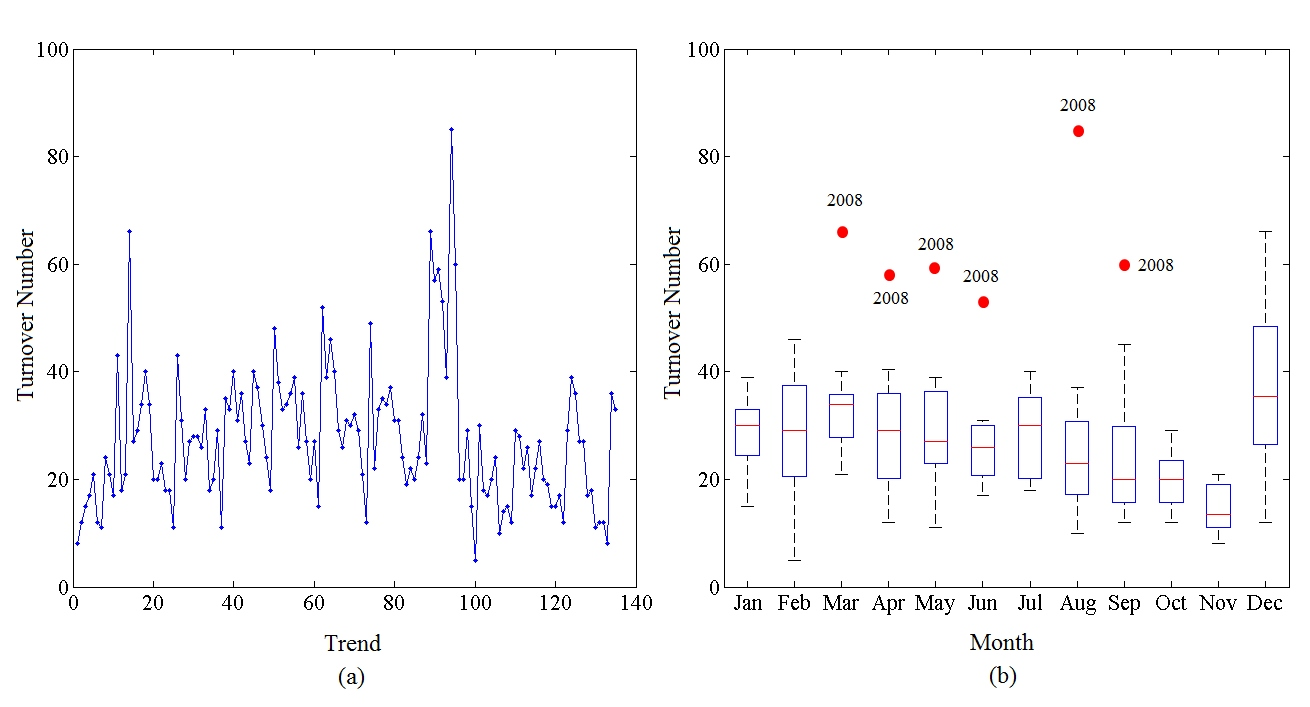
\includegraphics[width=5.5in]{Fig1.jpg}
	\caption{(a) Monthly Turnover Series Plotted Over Time and (b) Box Plot of Turnover Data.}
	\label{fig:1}
\end{figure}

\begin{figure}
	\centering
	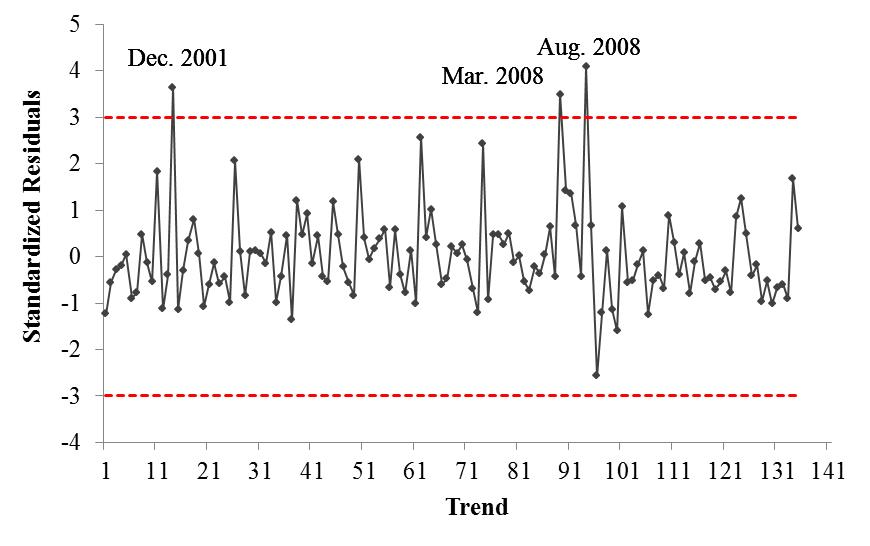
\includegraphics[width=5.5in]{Fig2.jpg}
	\caption{SPC Chart for Standardized Residuals.}
	\label{fig:2}
\end{figure}
The ACF and PACF plots for the turnover series are shown in Figure \ref{fig:3} (a, b). The pattern of unsmoothed data in the ACF and PACF hints at ARIMA(1,0,1) with some type of seasonality, but the seasonal pattern is not obvious.
\subsection{Cross-correlations}
The cross-correlation is employed between turnover series and CLI series to identify significant lag correlations. The cross-correlations between first differences for turnover and the CLI series were examined \citep{de1998}, and a “pre-whitening” process for the two series was used to identify the cross-correlation patterns \citep{box1970, bowie1981}.
% Department of Sciences at Pennsylvania State University, 2014).
Based all these calculation, CCFs from Lag 0 to Lag 8 are statistically significant, which indicates that the turnover series has statistically significant correlation with CLI and its 8 lags. The CLI and its 8 lags are applied into the dynamic regression, decomposition, and ARIMA model respectively as cyclical factor for forecasting.  

\begin{figure}
	\centering
	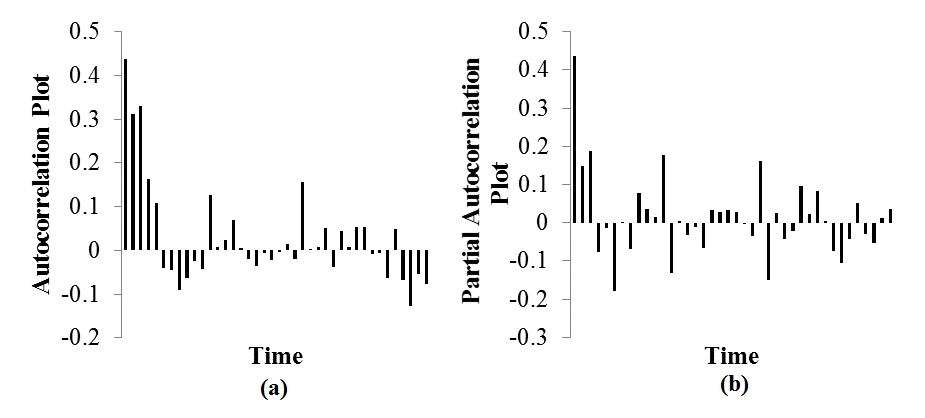
\includegraphics[width=5.5in]{Fig3.jpg}
	\caption{(a) Autocorrelation and (b) partial autocorrelation plots.}
	\label{fig:3}
\end{figure}


\subsection{Forecasting Results and Comparisons}
Forecasting evaluations for the time series models are provided in the Appendix Table \ref{tab:allmodels}, Table \ref{tab:dynamic}, Table \ref{tab:arima}, and Table \ref{tab:decomp}. Based on the evaluation statistics, 8 models are selected because of an acceptable $R^2$ value for the training and holdout data as well as their residual statistics that are the optimum among the other models (as shown in Table \ref{tab:1}).  On average, the holdout $R^2$ value of these models is 0.51 (range from 0.40 to 0.59). 
% Table generated by Excel2LaTeX from sheet 'Sheet1'
\begin{table}[htbp]
	\small %table fond
	\centering
	\caption{Statistics for Selected Time Series Models}
	\smallskip
	\begin{threeparttable}
		\begin{tabular}{C{2cm}p{0.5cm}m{5cm}C{0.8cm}C{1.5cm}ccc}%p: top m: middle
			\hline
			\multicolumn{1}{c}{Method} & \#    & \multicolumn{1}{c}{Model} & Pred $R^2$\tnote{1} & Holdout $R^2$& \multicolumn{1}{c}{MAPE}  & \multicolumn{1}{c}{Normality\tnote{2}} & \multicolumn{1}{c}{WN\tnote{3}} \\
			\hline
			\multirow{5}{2cm}{Univariate without external variable } & U1    & Regression with additive trend and seasonality & 0.51  & 0.57  & 26.15 & No    & No \\
			& U2    & Regression with additive trend, seasonality and intervention4  & 0.72  & 0.52  & 22.84 & Yes   & No \\
			& U3    & Decomposition & 0.65  & 0.54  & 17.97 & Yes   & Yes \\
			& U4    & WES with additive trend and seasonality & 0.52  & 0.52  & 20.65 & Yes   & Yes \\
			& U5    & ARIMA(1,0,1)(0,1,1) & 0.47  & 0.4   & 22.89 & Yes   & Yes \\  \hline
			\multirow{3}{2cm}{Univariate with external variable} & V1    & Dynamic regression using  lag7 CLI as predictor\tnote{4} & 0.77  & 0.59  & 19.91 & Yes   & Yes \\
			& V2    & Decomposition using  lag1 CLI as cycle & 0.65  & 0.55  & 17.97 & Yes   & Yes \\
			& V3    & ARIMA combining with lag1 CLI as cycle & 0.37  & 0.41  & 22.73 & Yes   & Yes \\
			\hline
		\end{tabular}%
		\begin{tablenotes}
			\item[1] Pred. $R^2$ is prediction $R^2$ value for training data.
			\item[2] Normality is residuals’ normality test.
			\item[3] WN is white noise test
			\item[4] The data is unsmoothed (or outliers are unadjusted) so as to take advantage of time series models that can accommodate interventions.
		\end{tablenotes}
	\end{threeparttable}
	\label{tab:1}%
\end{table}%

\subsubsection{Univariate Methods (	without External Variables)}
The regression model with additive trend and seasonality has the highest holdout$R^2$ (0.57) among the univariate models without external variables, indicating the model’s ability to explain 57\% of the total variation of the holdout sample. It is statistically significant ($P<0.05$) for the model and parameters. However, the residuals are not normally distributed and the model does not pass the white noise test. 

The regression model with additive trend, seasonality, and interventions (pulse and step) performs well with a training  $R^2$ of 0.72 and a holdout $R^2$ of 0.52, indicating the model’s ability to explain 72\% of the total variation of turnover for the training data and 52\% of the total variation of the holdout sample. It is statistically significant ($P<0.05$) for the model and parameters. The model has normally distributed residuals, but it does not have white noises. However, this regression model can capture the spike in December 2001 and sharp fluctuations from March 2008 to August 2008 (as shown in the Figure \ref{fig:4}). 
\begin{figure}
	\centering
	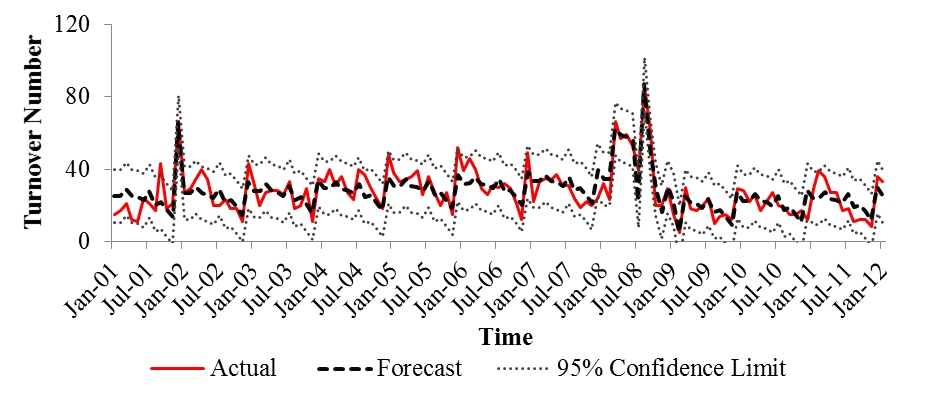
\includegraphics[width=5.5in]{Fig4.jpg}
	\caption{Regression with Interventions Forecast vs. Actual Turnover Number Plot.}
	\label{fig:4}
\end{figure}
The decomposition model is considered as the best univariate model without external variables because this model has a reasonably high training $R^2$ value (0.65), a good holdout $R^2$ value (0.54), and low MAPE (17.97). The residuals of this model are normally distributed and have a white noise pattern. Figure \ref{fig:5} shows the predicted turnover based on the decomposition model and the actual turnover number for holdout dataset. This plot validates the holdout performance of the decomposition model as it is able to mimic the changes in trend and seasonality of the turnover and prediction is close to the actual turnover numbers. However, it does seem to under-forecast for the 6 months June through November.
\begin{figure}
	\centering
	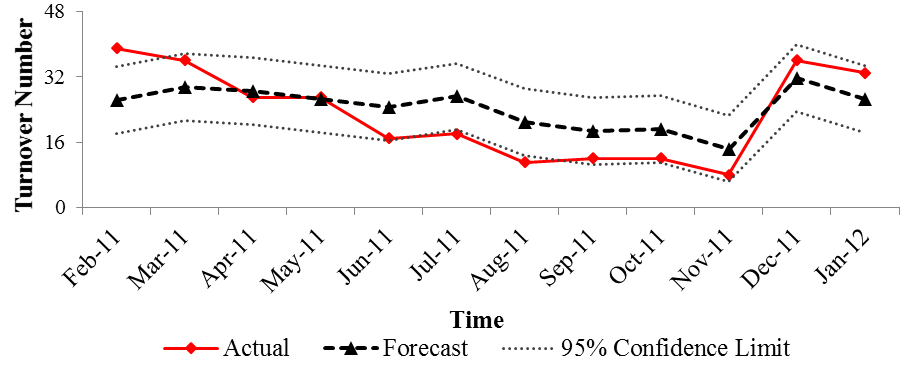
\includegraphics[width=5.5in]{Fig5.png}
	\caption{Decomposition Validation Forecast vs. Actual Turnover Number with Prediction.}
	\label{fig:5}
\end{figure}

\subsubsection{Univariate Methods (with External Variables)}
According to the cross-correlation analysis result, CLI and its 8 lags are applied in dynamic regression, decomposition model, and ARIMA(1,0,1)(0,1,1) respectively as external variable to forecast turnover number. The dynamic regression model with additive trend, seasonality, interventions (pulse and step), and lag7 of CLI is the best model among all models, since it has highest predicted and holdout  $R^2$ value (0.77 and 0.59), normalized residuals, and white noise. The dynamic regression is globally statistically significant and individually significant for the parameters ($P<0.05$).
\begin{figure}
	\centering
	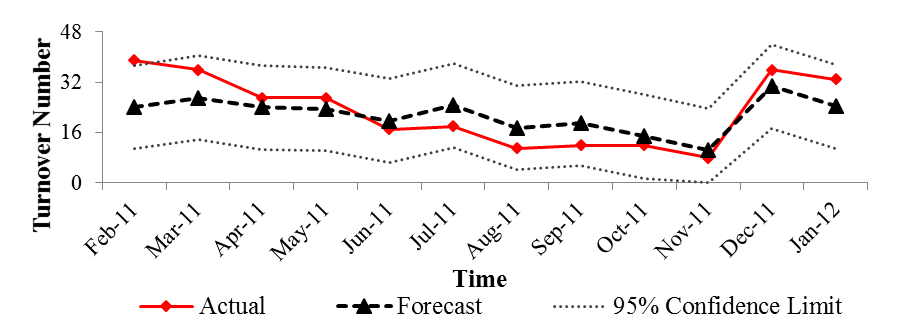
\includegraphics[width=5.5in]{Fig6.png}
	\caption{Dynamic Regression with Lag7 CLI Forecast vs. Actual Turnover Number for Holdout Dataset.}
	\label{fig:6}
\end{figure}
Figure \ref{fig:6} shows the predicted and actual turnover number plots for holdout dataset from dynamic regression model. Although there are under forecasts from July to September as well, the differences between forecasting value and actual value have become much tighter. Compared with top rated univariate methods without external variables, the performance of dynamic regression model is much improved after using CLI as an outside cyclical variable. 

\subsubsection{Nonlinear and Multivariate Methods (with External Variables)}
State space models with various combinations of errors, trend, seasonality, or an exogenous variable (CLI here) and VAR models of bivariate time series (turnover and CLI) are employed to forecast turnover number (as shown in Table 3). The exponential smoothing state space model with multiplicative error, no trend, and multiplicative seasonality has the highest holdout $R^2$ value (0.43) among all state space models, which is automatically selected by R forecast package from 27 exponential smoothing state space models. The residuals have white noise and are normally distributed. However, the training and holdout $R^2$ value (0.53 and 0.43) are relatively lower than the univariate regression models. 
Table 3 shows that the VAR models perform better than state space models. The VAR (4, constant, trend, and seasonality) is considered as the best among all these nonlinear and multivariate model with highest training and holdout $R^2$ value (0.62 and 0.64). The residuals are normally distributed and have white noise. However, variables in this model: lag terms of turnover and CLI are not statistically significant, indicating the model is over fitted. Only VAR (1, constant, trend, and seasonality) has significant lag 1 term of both turnover and CLI. This model also has higher training and holdout $R^2$ value (0.57 and 0.47) and white noise. However, its residuals are not normally distributed. 
The bivariate time series (turnover and CLI) does not have multivariate moving average pattern, which is not statistically significant. Therefore, the vector moving average (VMA) and vector autoregressive moving average (VARMA) methods are not employed to forecast. The volatility models (Garch (1,1) and stochastic volatility model) and nonlinear models (nonlinear autoregressive model and nonlinear threshold autoregressive model) have also been considered. However, all these models have lower training and holdout $R^2$ values and higher MAPE values. Their statistics are not provided in the Table \ref{tab:2} due to their poor performance.
\begin{table}[]
	\centering
	\caption{Statistics for Selected Nonlinear and Multivariate Models}
	\scriptsize
	\begin{threeparttable}
	\begin{tabular}{L{1.5cm}cL{3.5cm}ccccc}
		\toprule
		\multicolumn{1}{c}{Method} & \#    & \multicolumn{1}{c}{Model} & Pred. $R^2$ & Holdout $R^2$ & MAPE  & Normality & WN \\
		\midrule
		\multirow{6}[2]{*}{State Space} & S1    & Trend, Seasonality & 0.27  & 0.39  & 24.8  & No    & Yes \\
		& S2    & Trend, Slope, Seasonality & 0.23  & 0.32  & 28.58 & Yes   & Yes \\
		& S3    & Trend, Slope, Seasonality, CLI as regressor & 0.13  & 0.32  & 28.89 & Yes   & Yes \\
		& S4    & Exponential Smoothing (M,N,M) \tnote{1} & 0.51  & 0.43  & 21.14 & Yes   & Yes \\
		& S5    & Structural TS (Level, Slope)  & 0.46  & -0.16 & 22.82 & No    & No \\
		& S6    & Structural TS (Level, Slope, Seasonality)  & 0.51  & 0.04  & 21.47 & Yes   & Yes \\ \midrule
		\multirow{7}[2]{1.2cm}{Vector Autoregressive \tnote{2} } & VA1   & VAR(5, Constant, Seasonality) & 0.62  & 0.49  & 18.2  & No    & Yes \\
		& VA2   & VAR(5, Trend, Seasonality) & 0.63  & 0.52  & 18.37 & Yes   & Yes \\
		& VA3   & VAR(1, Constant, Trend, Seasonality) & 0.52  & 0.47  & 21.08 & No    & Yes \\
		& VA4   & VAR(2, Constant, Trend, Seasonality) & 0.59  & 0.44  & 19.63 & Yes   & Yes \\
		& VA5   & VAR(3, Constant, Trend, Seasonality) & 0.61  & 0.51  & 19.06 & Yes   & Yes \\
		& VA6   & VAR(4, Constant, Trend, Seasonality) & 0.62  & 0.64  & 18.44 & Yes   & Yes \\
		& VA7   & VAR(5, Constant, Trend, Seasonality) & 0.65  & 0.61  & 17.98 & Yes   & Yes \\
		\bottomrule
	\end{tabular}%
	\begin{tablenotes}
   \item[1]	M, N, M is multiplicative errors, no trend, multiplicative seasonality, respectively. 
   \item[2]	VAR(p) is pth order of  lag term. 
	\end{tablenotes}
	\end{threeparttable}
	\label{tab:2}%
\end{table}%
Even more non-linear and multivariate models were considered, but the intent of this research was not to go fishing for a best model but to find a simplistic model that could be used by human resource management (HRM).  It should be noted that a combination model might have been the better than our chosen dynamic regression model, but the authors were trying to keep it as simple as possible for HRM.
%%%%%%%%%%%%%%%%%%%%%%%%%%%%%%%%%%%%%%%
%%%%%    Time series analysis Conclusion  %%%%%%%%%%%%%%%%%%%
%%%%%%%%%%%%%%%%%%%%%%%%%%%%%%%%%%%%%%%
\section{Conclusion}
In this study, various univariate time series forecasting models for employee turnover prediction are tested and optimal models for In this paper, various time series forecasting models for employee turnover prediction are tested and optimal models for turnover forecasts are identified. The model in this paper actually performs better than those accessed in the literature review as a result of the external variable. Although VAR (4, constant, trend, and seasonality) has the highest holdout $R^2$, normally distributed residuals and white noise, dynamic regression model is concluded as the best forecasting model. There are several reasons why univariate methods are selected. In most cases, multivariate models help in generating more accurate model fit when compared to univariate models. However, univariate models are preferred as they are able to negate several drawbacks of multivariate models. For example, univariate models have less parameter uncertainty and less chance for outliers and errors due to their design simplicity. In most cases, univariate models are relatively easier to develop, interpret and get concrete conclusions. Multivariate models due to their complexity are more susceptible to misspecification. Besides, the explanatory variables in univariate models have to be determined accurately before forecasting the depending variable. Errors in forecasting the explanatory variable for a multivariate model may significantly affect the accuracy of the forecasts of the dependent variable when compared with an equivalent univariate model \citep{chatfield2000}. Apart from the benefits listed for univariate models, the dynamic regression model has several additional advantages. For example, an ARIMA error term which has autocorrelation pattern can be included in the model. Dynamic regression model is able to handle lagged regressors and various types of seasonalities. In addition, dynamic regression model can handle interventions or change points effectively, since these interventions or change points, such as holidays, promotions, new policy and so forth, are often common to the time series data. Thus, dynamic regression model could be used to forecast turnover for most of organizations of any size.  forecasts are identified. The model in the paper actually performs better than those accessed in the literature review. Dynamic regression model is concluded as the best forecasting model. Dynamic regression model has several advantages. For example, ARIMA error term which has autocorrelation pattern can be included in the model. Dynamic regression model is able to handle lagged regressors and various types of seasonality. In addition, dynamic regression model can handle interventions or change points effectively, since these interventions or change points, such as holidays, promotions, new policy and so forth, are often common to the time series data. Thus, dynamic regression model could be used to forecast turnover for most of organizations including small size, large size, and merged unit. However, to implement dynamic regression modelling, at least 5-years of monthly employee turnover data is preferred to make an accurate forecast. If the horizon of the dataset is less than 5 years, a special decomposition model \citep{ittig1997}could be considered as a substitute. Even though the forecasting horizon provided by dynamic regression model is relatively short, this is not a big issue for HR departments, since most of HR departments are only interested in a short term, such as three months, forecast. Therefore, if the HR department in an organization is not well familiar with forecasting techniques, dynamic regression model could be a good option for a preliminary turnover forecast once a CLI can be identified as in this paper. 

It is worth mentioning that an external variable like CLI in this paper does help in forecasting turnover since it does anticipate cyclical turning points. Incorporating such an external variable in the model is very helpful to get a good forecast when the HR department has a small and unreliable data set. Incorporating external variables, such as CLI, may help the whole forecasting process. If an external variable such as CLI is not available, a decomposition model could be considered as the first choice rather than dynamic regression model. In practice, some software such as NCSS or MINITAB have an embedded decomposition macro, which the HR departments could easily run given they knew how to estimate the cyclical variation.
\subsection{Practical implications}
\begin{itemize}
\item[(1)]	According to our findings, employee turnover forecast, in practice, could be handled easily. We suggest that HR departments could use regression model for the preliminary forecast and the accuracy of forecast is acceptable. However, there are some types of interventions that regression cannot handle, such as pulse or steps with exponential decay or growth. Dynamic regression is likely to be used as an alternative for forecasting.
\item[(2)] In this study, statistical analysis packages SAS and NCSS are used for the forecast. However, to some organizations, the HR departments are unwilling to spend extra funding on software purchase. Under this circumstance, Microsoft Excel could be a good alternative for the time series forecast without extra investment, because there have been some open source time series forecasting packages designed to run under Excel environment in the market. The forecasting models such as naïve model, moving average, exponential smoothing, decomposition, regression, and ARIMA model have been included into these packages \citep{warren2008}.
\item[(3)]	Another option these days is to use R for the dynamic regression \citep{hyndman2014}. The pseudo R code for dynamic regression and test on residuals (normality and white noise test) is provided below. 
\begin{lstlisting}
## Install R package
library (dynlm)
library (normwhn.test)
## Turnover is turnover data.  
## Trend is a continuous variable with value from 1 to n. 
## Seasonality is a dummy variable representing seasonal periods. 
## X is the lag term of CLI.
## Intervention is the external variable impact: yes=1 and no=0.
## Build model ## Load dataset
Turnover = read.xls (“turnover_data_in_excel.xls”)
## IMPORTANT: Some R codes in dynamic regression may not handle fancy intervention analysis.
Turnover.Model = dynlm (Turnover ~ Trend + Seasonality + L(CLI, X) + Intervention) 
## Model summary
summary ( Turnover.Model)
## Calculate residuals
Residual = resid (Turnover.Model)
## Normality test on residuals
normality.test1 (Residual)
## White noise test on residuals
whitenoise.test (Residual)
\end{lstlisting}
\end{itemize}
\subsection{Limitations and future research}
This study is limited to forecast total turnovers in an organization. It may be possible to apply univariate time series forecasting models to forecast turnovers in different categories like retirement or volunteer quit. Although the study incorporated CLI as an external factor and the accuracy of forecasts is well improved, the external factors affecting turnover can be much beyond the scope of CLI, as local and cyclical economic fluctuations strongly influence the propensity of employees to quit \citep{abelson1984}.


    \chapter{Survival analysis} \label{ch:surv}
\section{Methods}
The time series approaches provide a good prediction on turnover based on organizational level. However, more questions are brought to the forefront, like when a specific employee will turnover, what factors affect employee's turnover, why they will turnover: voluntary quit, retire, or by other reasons. And also the dataset has two kinds of unknown information. There are active employees who are hired from November 1st, 2000 to July 12th, 2012, and terminative employees who left the organization from November 1st, 2000 to July 12th in the dataset. The turnover date for active employees who left after July 12, 2012 and the information for terminative employee who left before November 1st, 2000 are both not available. These two kinds of  unknown information cause two kinds of bias: right censoring and left truncation. Besides, there is an intervention event implemented by HR in 2008 which is a downsizing policy to incent the employees who are eligible for retirement to retire. Therefore, how to model this incentive and to estimate its effect are another interesting questions. All these questions and problems can be solved by lifetime analysis, also called survival analysis. The cox proportional hazard model is to build the forecasting model, to generate a base line, and to identify significant factors for turnover. Competing risks analysis is used to answer what kind of reasons cause employees  turnover. A time dependent covariates is created for year 2008 to model the incentive effect and to achieve more accurate forecasting result. Finally, a simulation study is performed to examine the forecasting capability of cox proportional hazard model on the left truncation and right censor dataset.
\subsection{Right censoring and left truncation}
Right censoring and left truncation are common in survival analysis. The right censoring is that the main event of interest (failure) occurs after the study window. Let $T$ denotes the time of main event of interest to occur and let $C$ denotes the end time of study. An observation is right censored when $T> C$, indicating the study do not have the failure time of the right censored observation. In this study, the study window is from November 1st, 2000 to July 12th, 2012. Thus, employees who leave the organization after the study window are right censored. These right censored observations require special treatment in survival analysis: a censor indicator variable is created: 
\begin{align*}
\delta_i&=
\begin{cases}
1   &\text{if  }  t_i \leq c_i \text{ (uncensored),}\\
0   &\text{if  }  t_i > c_i \text{ (censored),}
\end{cases}
\end{align*}
where, $i$ denotes the ith observation, and the failure time of event for ith observation is minimum time between $t_i$ and $c_i$, i.e., $min(t_i, c_i)$, that is when $ c_i <t_i $, $c_i$ is taken as end time of the ith observation in order to do next  analysis.

Left truncation is that the occurrence of an intermediate event prior to the main event of interest appear in the sample dataset. Left truncation in this study occurs when employees enter to the organization at random time, that is, the hired time precedes the origin of the study window. Then, the employees are followed from this entry time until the turnover events occur or until they are right-censored. So, the employees turnover before the entry time of the study will not be aware or not be in the sample dataset. Let $T$ denotes the time of main event of interest to occur and let $X$ denotes the time an individual enters the study, that is time of truncation events occurs. Only the individuals with $T \geq X$ are observed in the study window. The left truncation leads to the bias in the analysis. For example, employees who entered the company in 1950s, appear to stay longer as compared the employees entered in 1960s or later, causing by the fact that the sample dataset does not include the observation recorders for the employees who left the organization before November, 2000. The existence of truncation in the data must be taken into account in order to overcome this bias and to achieve accurate estimation of survival analysis \citep{carrion2010}. Let $t_{i0}$ denotes the start time of the ith observation, i.e., hired time or age at hired of ith employee, $x_{i}$ denotes the entry time of the ith observation, i.e., the start time of study (November 1st, 2000) or age at November 1st, 2000. The start time of the observation is maximum value between $t_{i0}$ and $x_i$, that is when $t_{i0} < x_i $, $x_i$ is taken as start time of the ith observation in order to eliminate the left truncation bias \citep{allison1995}. The number of failures in the $t_j$ is redefined for left truncation. When $x_i < t_j \le t_i$, the observation is in the risk set. When $t_{j} < x_i \le t_i$, the ith observation has not entered study yet at $t_j$ and it cannot be considered in the risk set. When $x_i \le t_i < t_j$, it indicates the ith observation whose failure time before $t_j$, and it cannot be considered in the risk set at time $t_j$ neither \citep{carrion2010}.
%%%%%%%%%%%%%%%%%%%%%%%%
%%%%%%%%%%%%%%%%%%%%%%%%
%%%%%%%%%%%%%%%%%%%%%%%%

\subsection{Cox proportional hazard regression}
Cox proportional hazards regression is a widely used method for estimating survival distributions. It was introduced in a seminal paper by \citet{cox1972}. The Cox PH model is usually taken the form of hazard model formula shown \ref{eq:cox}:
\begin{equation}
\label{eq:cox}
h(t,x)=h_0(t)e^{(\sum_{i=1}^{k}\beta_ix_i)}
\end{equation}

where $x=(x_1, x_2, \ldots, x_k)$, $h_0(t)$ is the baseline hazard occurring when X=0, $\beta$ is the coefficients of $x$. 
The model provides a hazard expression at time t for an individual with a given specification of a set of explanatory variables denoted by the $x$. The Cox PH formula is the product of quantities at hazard time $t$: $h_0 (t)$ as the baseline hazard function and the exponential expression to the linear sum of $\beta_i x_i$, where the sum is over the $k$ explanatory $X$ variables. $x$ can be time-independent covariates, because it does not involve time $t$, or time-dependent covariates which Cox PH model is called the extended Cox model. Because the baseline hazard function $h_0 (t)$ is an unspecified function, the Cox PH model is a semiparameric model, whose estimation can closely approximate correct parametric model \citep{kleinbaum1998}, causing the semiparameric model is "robust" and popular. Taking the logarithm of both sides of the equation, the Cox PH model is rewritten in equation \ref{eq:coxlog}:
\begin{equation}
\label{eq:coxlog}
\log{h(t,x)}=\alpha(t)+\sum_{i=1}^{k}\beta_ix_i 
\end{equation}
where $\alpha(t)=\log{h_0(t)}$. If $\alpha(t)=\alpha$, the baseline is exponential distribution and the model is exponential model. In Cox PH model, $\alpha(t)$ do not limited on specific parametric distributions and it can take any form. The partial likelihood method is used to estimated $\beta$ coefficients of the Cox model without having to specify the baseline \citep{allison1995}.
%%%%%%%%%%%%%%%%%%%%%%%%
%%%%%%Time dependent %%%%%%%%%%
%%%%%%%%%%%%%%%%%%%%%%%%
\subsection{Time dependent covariate}
Time dependent covariate depicts that a covariate is not necessarily constant through the whole study and change values over the course of the observation. The extended Cox model incorporates both time-independent and time-dependent covariates as shown in equation \ref{eq:timecovar}:
\begin{equation}
\label{eq:timecovar}
h(t,x)=h_0(t)e^{(\sum_{i=1}^{k_1}\beta_ix_i+\sum_{j=1}^{k_2}\gamma_jx_j(t))}
\end{equation}
where $x=(x_1, x_2, \ldots, x_{k_1}, x_1(t), x_2(t), \ldots, x_{k_2}(t))$, $h_0(t)$ is the baseline hazard occurring when $x=0$, $\beta$ and $\gamma$ are the coefficients of $x$. 
%%%%%%%%%%%%%%%%%%%%%%%%
%%%%%%Competing risk analysis%%%%%%%%
%%%%%%%%%%%%%%%%%%%%%%%%
\subsection{Competing risks analysis}
A competing risk is an event whose occurrence either precludes the occurrence of the event of interest or fundamentally alters the probability of occurrence of this event of interest \citep{tableman2003}. For example, turnover causes of an employee are exclusive and independent, i.e. an employee can experience only one event such as voluntary quit rather than retirement. This alters the probability of experiencing the event of interest, like retirement. Such events are known as competing risks events where one event of several different types of possible events can occur and hence the survival analysis for each event is calculated separately with the other events set as censored. Two mutually exclusive causes are considered as the event of interests for each employees in this study, which are voluntary quit and retirement. And the other events are treat as censored.

The reason for studying retirement and voluntary quit is because the organization are interested in forecasting the turnover of retirement of voluntary quit. There are $1/3$  employees in that organization are over 50 years old who are eligible for retirement. The employee for voluntary quit usually is the one organization would not like to leave \citep{allen2010}. And voluntary quit costs highly for the organizations and firms \citep{selden2000}. The other reasons of turnover, such as layoff, transfer, death, or disability are not considered, because the factors causing the occurrence of these turnover are random and hard to predict. The Cox PH models for competing risks as shown in equation \ref{eq:competing}:
\begin{equation}
\label{eq:competing}
h_j(t,x)=h_{j0}(t)e^{(\sum_{i=1}^{k}\beta_{ij}x_i)}
\end{equation}
where, $x_{j}$ is the covariate for a specific type of turnover. Note that the coefficient $\beta$ is the effects of the covariates may be different from different turnover types. If $\beta_{ij}$  is the same for all j, the model simplified to Cox PH model as shown in equation \ref{eq:cox}. 
%%%%%%%%%%%%%%%%%%%%%%%%%%%
%   Data preparation
%%%%%%%%%%%%%%%%%%%%%%%%%%
\subsection{Data preparation}
The dataset is split into two datasets by time point November 1st 2010: training and holdout. The training part is used to build the model (November 1st, 2000 - October 31th, 2010), and the holdout part is to validate the model performance (November 1st, 2010 - July 12, 2012). Age of employees is used to build the model as dependent variable rather than the length of service time in the organization. The age is calculated based on two time points: start age and leaving age. Start age is the age of an employee at hired in the organization, or the age at November 1st 2000, when the employee was hired before November 1st, 2000; leaving age is the age at the date who left the organization or the age at October 31st 2010, if the employee was still working in the organization at that time which are treated as censored data. The covariates identified from the turnover dataset and used to build the final model are payroll, gender, organization level, cocs code, age at hired, year of service at hired, termination date and termination type: 
\begin{itemize}
	
	\item Payroll (PR): hourly, weekly, or monthly payroll, 
	\item COCS code: Crafts(C), Engineers (E), General Administrative (G), Laborers (L), General Managers (M),  Administrative (P),  Operators (O), Scientists (S), Technicians (T))
	\item Gender: male, female
	\item Age at hired: most recent age when an employee is hired.
	\item Age at started: the age of an employee at November, 2000, if employee hired before November, 2000, or the age of an employee at hired, if employee hired after November, 2000. 
	
	\item Years of service at hired (YCSH): the years of service which accounts for pension plan when employee is most recently hired.
	\item Termination date: the date when an employee left the organization.
	\item Termination type: the reasons for employees leaving the organization, such as retirement(RE),  volunteer quit (VQ), and other reasons. 
	\item Age at end: the age of an employee at termination date, if employee left the organization before October 31th, 2010, or the age of an employee at October 31th, 2010.
	\item Organization level (ORG): the divisions of the organization.
\end{itemize}
A time-dependent covariate (policy) is created to model the incentive for 2008. Time dependent covariate is a dummy variable:
\begin{align*}
Policy&=
\begin{cases}
1   &\text{if employee works in year 2008 }\\
0   &\text{if  employee does not work in year 2008}
\end{cases}
\end{align*}
%%%%%%%%%%%%%%%%%%%%%%%%
%%%Model evaluation and variable selection%%%%
%%%%%%%%%%%%%%%%%%%%%%%%

\subsection{Model evaluation and variable selection}
The training dataset is applied to Cox PH model to build employee working lifetime distribution utilizing individual demographic information. Then the coefficients of covariates and the baseline from the model are used to calculated the turnover probability for each employee as shown in equation \ref{eq:prob}. 
\begin{equation}
\label{eq:prob}
\begin{split}% to allgin the equation
P\{t_{j-1}<T<t_j\} &=1-P\{T>t_j|T \ge t_j\}\\
&=1-\frac{S_{t_j}}{S_{t_{j-1}}}   \\
&=1-\frac{{S_0(t_j)}^{(\sum_{i=1}^{k}\beta_ix_i)}}{   {S_0(t_{j-1})}^{(\sum_{i=1}^{k}\beta_ix_i)}}
\end{split}
\end{equation}
where, $T$ is survival time, $t_j$ is a specific value for $T$, $S_0(t)$ is the baseline function generated by Cox PH model, $x$ is the covariates, and $\beta$ is the coefficient.
The expected turnover number is achieved by the summation of turnover probability for all the active employees at $t_j$ as shown in \ref{eq:expturnover}.  
\begin{equation}
\label{eq:expturnover}
E(\text{turnover number at } t_j)=\sum_{i=1}^k{P_i\{t_{j-1}<T<t_j\}} 
\end{equation}
where, $i$ denotes the ith observation. -2 log likelihood statistic, Akaike’s information (AIC) and Schwartz’s Bayesian criterion (SBC) are applied to evaluate model performance and select variables. The variable selection procedure is manually backwards selection. First, put all the variables into the model. Second, remove one non-significant variable ($P>0.05$) and rerun the model again to compare AIC and SBC value with those value of previous model. If there is no or very small difference between current and previous model, the model selection stops and the variables in the model are selected variables. Otherwise, repeat the second step. The evaluation step is to calculate the yearly predicted turnover number for training and holdout dataset, and then compared the predicted number with the actual number. The survival analysis is performed on software SAS and R package.
%add evaluation formula.
%%%%%%%%%%%%%%%%%%%%%%%%
%%%Simulation on left truncation and right censor%%%%
%%%%%%%%%%%%%%%%%%%%%%%%
\subsection{Simulation on left truncation and right censor}
The simulation is used to examine Cox PH model predictive performance with right censoring and left truncation. The generation  of simulation lifetime data is based on the Weibull distribution. %The hazarld function for Weibull regression model with shape parameter $\alpha$, scale parameter $\lambda$, and covariate $X$ is shown in equation \ref{eq:weibul}, given $h_0=\alpha(\lambda)^\alpha t^{\alpha-1}$: 
%\begin{equation} \label{eq:weibul}
%\begin{split}% to allgin the equation
%h(t|X) & =h_0(t)exp(\beta X) \\
%         &=\alpha (\lambda (exp(\beta X)^{\frac{1}{\alpha}})^\alpha t^{\alpha-1} \\
%         &=\alpha(\tilde{\lambda} )^\alpha t^{\alpha-1}
%\end{split}
%\end{equation}
%where, $\tilde{\lambda}=\lambda (exp(\beta X)^{\frac{1}{\alpha}}$.
The simulation can be described as follows. The sample size was n=4000, with one variable $X$, named Age, which follows uniform distribution with parameter $a$ $(a=22)$ and $b$ $(b=70)$. Only one variable age is used in simulation process to make the estimation procedure simple and close to real world. The coefficient $\beta_{age}$ is taken $-0.025$ and $\beta_0=1.5$. 
Then, the survival time $T$ is random generated for each observation based on Weibull distribution with shape parameter $\alpha$ and scale parameter $\lambda$, where $\alpha=1.5$ and $\lambda=exp(-0.025age+\beta_0)^{\frac{1}{\alpha}}$.

The simulation is performed on right censoring and left truncation separately, in order to observe the effects for different bias.  
For right censoring simulation, the start point for all the observations are set as 0, and stop point is equal to the survival time $t_i$ for ith observation where $T=(t_1, t_2, \ldots, t_n)$. After that, a survival time histogram is generated. The censor time $C$ is set as first quarter, median, third quarter, and maximum of the survival time, respectively, to get 75\%, 50\%, 25\% and 0\% censoring proportions. When the survival time $t_i$ for ith observation is not greater than the censor time ($c_i$), the stop point is survival time and censor variable $\delta_i$ is 1. When survival time $t_i$ for ith observation is greater than censor time ($c_i$), the stop point is change to censor time ($c_i$) and censor variable $\delta_i$ is  0. The start point and the stop point are dependent variable in the cox regression model. $\delta$ is censor variable. And variable age is predictor or covariate. All these variables are applied to cox model using R EHA package. 

For left truncation simulation, the start point $U$ is generated as uniform distribution with $a=0$ and $b=max(T)$ which indicates an observation start randomly from time 0 to time $max(T)$. The stop point $S$ is $U+T$. The histogram is generated for $S$. The truncation time $L$ is set as 0, first quarter, median, and third quarter of $S$, respectively, to get 0\%, 25\%, 50\%, and 75\% truncation proportions. When start point $u_i$ for ith observation is less than truncation time $l_i$, the start point is reset as truncation time $l_i$. When start point $u_i$ for ith observation is not less than truncation time $l_i$, the start point does not change ($u_i$). In left truncation, the censor variable $\delta$ for all the observations are equal 1. All these variables are also used to build Cox PH model in R EHA package. The Cox PH model is conducted using "phreg" function in eha package and using weibull distribution to estimate the baseline for both right censoring and left truncation simulation. The "phreg" function performs Cox PH model and also provides a parametric baseline hazards estimation \citep{brostrom2012}. Total predicted failure number is calculated as shown in equation \ref{eq:prob} and \ref {eq:expturnover}. The actual and forecast failure number are plotted to compare the effects on different levels of bias.

%accelarate model%

%%%%%%%%%%%%%%%%%%%%%%%%%%%
%%%%%%%%%%%%%%%%%%%%%%%%%%%
%%%                           Result              %%%%%%%%%%
%%%%%%%%%%%%%%%%%%%%%%%%%%%%


%%%%%%%%%%%%%%%%%%%%%%%%%%%
%%%%%%%%%%%%%%%%%%%%%%%%%%%
%%%                       Simulation   Result              %%%%%%
%%%%%%%%%%%%%%%%%%%%%%%%%%%
\section{Survival analysis results}
\subsection{Cox PH Model Analysis Result without Time-dependent Covariate}
A turnover model for entire organization is built by survival analysis.  Table \ref{tab:fit1} indicates that the accuracy of cox model fit is improved after adding covariates, as the -2 log Likelihood value, AIC and SBC value decrease with covariates. The model is statistically significant as all the p-values are less than 0.05 with 19 degrees of freedom. Table \ref{tab:variable1} shows the variables: payroll(PR), organization level (ORG), COCS code, age at start, and year of service at hired (YCSH) are statistically significant and cannot be eliminated from the model due to significant p-values. The test has nine degrees of freedom (df), corresponding to the nine coefficients that are estimated for ORG and six degrees of freedom corresponding to the six coefficients that are estimated for COCS. This test is the overall test for each variable which is omitted the category. Table \ref{tab:para1} shows the parameter estimates and the hazard ratio for each variable. Parameter estimates shows the coefficients estimates and associated statistics. Notice that there is no intercept estimate in Cox PH model. There are eight lines for the COCS variable. The first six lines contain coefficients, standard errors, and hypothesis tests for level 1 to level 6 of COCS, while the last two lines informs us that level 7 and level 8 are the omitted category. Hence, each of the estimated coefficients is a contrast with reference group of level 9. For categorical variables, the hazard ratio is the ratio of the current group to the reference group, which almost exactly like odds ratio in logistic regression. The hazard ratio for payroll 1 (monthly payroll) is 0.71, indicating that the hazard of leaving the organization for those with monthly payroll is only about 71 percent of the hazard for those with hourly payroll ( adjusted with other covariates). For the continuous variable like Age at start, the hazard ratio is 0.81, which yields 100(0.81-1)=-19, indicating that for each 1-year increase in the age at start for an employee, the hazard of leaving goes down by an estimated 19\%. The different hazard ratios for ORG levels indicate the different turnover behaviors among organization level. The different hazard ratios for COCS indicate the different turnover behaviors among different job classification. Besides, the hazard ratios of Age at start, YCSH are all less than 1, indicating that an employee hired with certain age and years of service are less likely to leave the organization than a new employee with young age and 0 years of service.
\begin{table}[htbp]
	\small
	\centering
	\caption{Model Fit Statistics}
	\begin{tabular}{rrr}
		\hline
		\multicolumn{1}{c}{Criterion} & \multicolumn{1}{c}{Without Covariates} & \multicolumn{1}{c}{With Covariates} \\
		\hline
		-2 LOG L & \multicolumn{1}{c}{46130.96} & \multicolumn{1}{c}{41978.58} \\
		AIC   & \multicolumn{1}{c}{46130.96} & \multicolumn{1}{c}{42016.58} \\
		SBC   & \multicolumn{1}{c}{46130.96} & \multicolumn{1}{c}{42132.62} \\
		\hline
	\end{tabular}%
	\label{tab:fit1}
\end{table}%

% Table generated by Excel2LaTeX from sheet 'Sheet2'
\begin{table}[htbp]
	\small
	\centering
	\caption{Variables Statistics Test}
	\begin{tabular}{cccc}
		\hline
		Effect & DF    & Wald $\chi^2$ &  Pr>$\chi^2$ \\
		\hline
		PR    & 2     & 9.2717 & 0.0097 \\
		ORG   & 9     & 1930.686 & $<.0001$ \\
		COCS  & 6     & 25.0608 & 0.0003 \\
		Age at start  & 1     & 673.0102 & $<.0001$ \\
		YCSH  & 1     & 640.4862 &$ <.0001$ \\
		\hline
	\end{tabular}%
	\label{tab:variable1}
\end{table}%
% Table generated by Excel2LaTeX from sheet 'Sheet2'
\begin{table}
	\centering
	\small
	\caption{Cox PH model parameter estimates}
	\begin{tabular}{cccccccc}
		\hline
		Parameter & Label & DF    &  Estimates & Std. Error & $\chi^2$    &  $Pr>\chi^2$ & Hazard Ratio \\
		\hline
		PR    & PR 1  & 1     & -0.346 & 0.134 & 6.64  & 0.01  & 0.71 \\
		PR    & PR 2  & 1     & -0.226 & 0.095 & 5.71  & 0.02  & 0.80 \\
		ORG   & ORG 1 & 1     & 3.465 & 0.381 & 82.77 & $<.0001$ & 31.98 \\
		ORG   & ORG 2 & 1     & 2.464 & 0.383 & 41.50 & $<.0001$ & 11.75 \\
		ORG   & ORG 3 & 1     & 2.012 & 0.393 & 26.21 & $<.0001$ & 7.48 \\
		ORG   & ORG 4 & 1     & 2.203 & 0.385 & 32.69 & $<.0001 $& 9.06 \\
		ORG   & ORG 5 & 1     & 2.378 & 0.399 & 35.53 & $<.0001$ & 10.78 \\
		ORG   & ORG 6 & 1     & 2.302 & 0.397 & 33.58 & $<.0001$ & 9.99 \\
		ORG   & ORG 7 & 1     & 4.461 & 0.381 & 137.28 & $<.0001$ & 86.60 \\
		ORG   & ORG 8 & 1     & 4.628 & 0.384 & 145.23 & $<.0001$ & 102.28 \\
		ORG   & ORG 9 & 1     & 3.780 & 0.383 & 97.69 & $<.0001$ & 43.83 \\
		Cocs  & Cocs 1 & 1     & -0.041 & 0.074 & 0.30  & 0.59  & 0.96 \\
		Cocs  & Cocs 2 & 1     & 0.194 & 0.126 & 2.37  & 0.12  & 1.22 \\
		Cocs  & Cocs 3 & 1     & -0.011 & 0.095 & 0.01  & 0.91  & 0.99 \\
		Cocs  & Cocs 4 & 1     & 0.117 & 0.086 & 1.85  & 0.17  & 1.12 \\
		Cocs  & Cocs 5 & 1     & 0.018 & 0.126 & 0.02  & 0.89  & 1.02 \\
		Cocs  & Cocs 6 & 1     & -0.101 & 0.123 & 0.67  & 0.41  & 0.90 \\
		Cocs  & Cocs 7 & 0     & 0.000 & .     & .     & .     & . \\
		Cocs  & Cocs 8 & 0     & 0.000 & .     & .     & .     & . \\
		Age at start  &       & 1     & -0.208 & 0.008 & 673.01 & $<.0001$ & 0.81 \\
		YCSH  &       & 1     & -0.069 & 0.003 & 640.49 & $<.0001$ & 0.93 \\
		\hline
	\end{tabular}%
	\label{tab:para1}
\end{table}%


\begin{figure}[htbp]
	\centering
	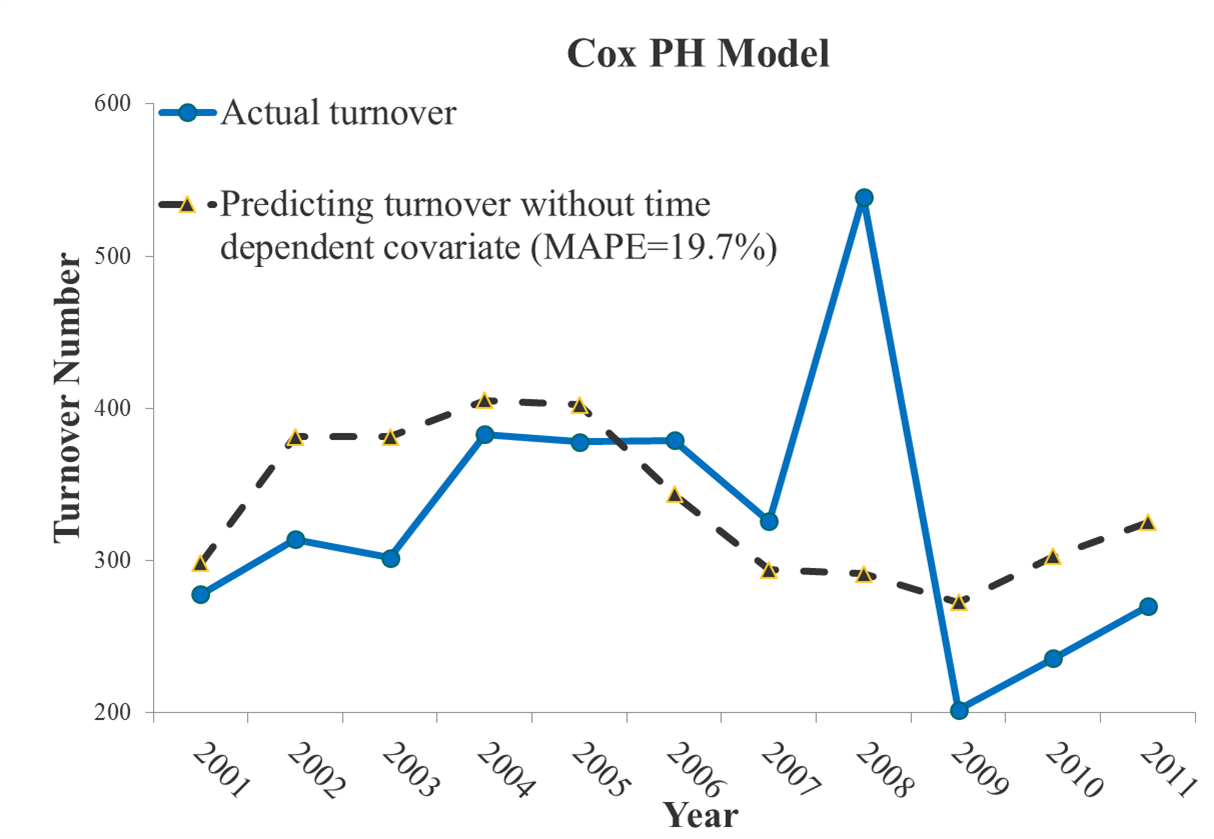
\includegraphics[width=5.5in]{Fig8.png}
	\caption{Actual vs. predicted turnover number for Cox PH model}
	\label{fig:8}
\end{figure}
All the data including training and holdout dataset are calculated the expected turnover number. The data for 2011 is holdout data set. The model performance as shown in Figure \ref{fig:8} is reasonable for the time period between 2004 and 2007 as the variation between them is quite insignificant. The model underestimates 2008 and overestimates after 2008 onwards. Year 2008 turnover number is much larger than the other years, because of an incentive policy published in that year leading to an increase in employee turnover in that year.  A new model with time-dependent covariates  has to be considered to accommodate the intervention event of year 2008.
%%%%%%%%%%%%%%%%%%%%%%%%%%%%
%%%%%%%%%%%%%%%%%%%%%%%%%%%%%%%%
%%%%%%%%%%%%%%%%%%%%%%%%%%%%%%%%
%%%%%%%%%%%%%%%%%%%%%%%%%%%%%%%%
\subsection{Cox PH Model with Time-dependent Covariate}
A time-dependent covariate (policy) is applied to model the intervention for 2008. It is a significant difference for AIC values before and after policy adding into the model and also the p-value is less than 0.05. Therefore the policy cannot be removed from the model. The variables: Payroll, ORG, YCSH, Age at Start all make a significant difference for the model without covariates and also statistically significant due to small p-values. Thus, they are all applied into the model. However, the variable COCS and Gender are not statistically significant due to the p-value larger than 0.05. These two variables can be removed from the model. Table \ref{tab:fit2} shows the model is statistically significant and Table \ref{tab:var2} indicates all the variables:  Policy, PR (payroll), YCSH (years of service at hired), ORG (organization level) and Age at start) are statistically significant with p-value less than 0.05. Table \ref{tab:para2} shows the parameter estimates and statistics for Cox PH model with variable policy. The hazard ratio for policy$=1$ is 3.18 indicating that the hazard of employees leaving the organization with an incentive policy is only about 318\% percent of the hazard without the incentive policy (adjusted with other covariates). After plotting the actual and predicted turnover number, the intervention is captured by the adjusted model in 2008 as clearly shown in the Figure \ref{fig:9}. Therefore, this model preforms better than the model without time-dependent covariate.  

% Table generated by Excel2LaTeX from sheet 'w time-covar'
\begin{table}[htbp]
	\small
	\centering
	\caption{Model Fit Statistics}
	\begin{tabular}{rrr}
		\hline
		\multicolumn{1}{c}{Criterion} & \multicolumn{1}{c}{Without Covariates} & \multicolumn{1}{c}{With Covariates} \\
		\hline
		-2 LOG L & \multicolumn{1}{c}{45729.81} & \multicolumn{1}{c}{41251.60} \\
		AIC   & \multicolumn{1}{c}{45729.81} & \multicolumn{1}{c}{41279.60} \\
		SBC   & \multicolumn{1}{c}{45729.81} & \multicolumn{1}{c}{41364.99} \\
		\hline
	\end{tabular}%
	\label{tab:fit2}%
\end{table}%

% Table generated by Excel2LaTeX from sheet 'w time-covar'
\begin{table}[htbp]
	\small
	\centering
	\caption{Variables Statistics Test}
	\begin{tabular}{cccc}
		\hline
		Effect & DF    & Wald $\chi^2$ &  $Pr>\chi^2$ \\
		\hline
		ORG   & 9     & 2075.926 & $<.0001$ \\
		YCSH  & 1     & 663.0154 & $<.0001$ \\
		PR    & 2     & 46.7408 & $<.0001$ \\
		Policy & 1     & 380.682 & $<.0001$ \\
		Age at start  & 1     & 457.5078 & $<.0001$ \\
		\hline
	\end{tabular}%
	\label{tab:var2}%
\end{table}%

% Table generated by Excel2LaTeX from sheet 'w time-covar'
\begin{table}[htbp]
	\small
	\centering
	\caption{Cox PH Model Parameter Estimates with Variable Policy}
	\begin{tabular}{cccccccc}
		\hline
		Parameter & Label & DF    &  Estimate & Std. Error & $\chi^2$    & $ Pr>\chi^2$ & Hazard Ratio \\
		\hline
		ORG   & ORG 2 & 1     & -0.989 & 0.073 & 185.051 & $<.0001$ & 0.372 \\
		ORG   & ORG 3 & 1     & -1.369 & 0.115 & 141.977 & $<.0001$ & 0.254 \\
		ORG   & ORG 4 & 1     & -1.244 & 0.086 & 210.286 & $<.0001$ & 0.288 \\
		ORG   & ORG 5 & 1     & -1.046 & 0.133 & 61.462 & $<.0001$ & 0.351 \\
		ORG   & ORG 6 & 1     & -1.145 & 0.129 & 79.078 & $<.0001$ & 0.318 \\
		ORG   & ORG 7 & 1     & 1.169 & 0.059 & 387.254 & $<.0001$ & 3.22 \\
		ORG   & ORG 8 & 1     & 1.354 & 0.075 & 323.271 & $<.0001$ & 3.872 \\
		ORG   & ORG 9 & 1     & 0.304 & 0.066 & 21.182 & $<.0001$ & 1.355 \\
		ORG   & ORG 10 & 1     & -3.553 & 0.410 & 75.108 & $<.0001$ & 0.029 \\
		YCSH  &       & 1     & -0.071 & 0.003 & 663.015 &$<.0001$ & 0.932 \\
		PR    & PR 1  & 1     & -0.323 & 0.047 & 46.680 & $<.0001$ & 0.724 \\
		PR    & PR 2  & 1     & -0.239 & 0.061 & 15.186 & $<.0001$ & 0.787 \\
		Policy & policy 1 & 1     & 1.157 & 0.059 & 380.682 & $<.0001$ & 3.18 \\
		Age at start &       & 1     & -0.183 & 0.009 & 457.508 & $<.0001$ & 0.833 \\
		\hline
	\end{tabular}%
	\label{tab:para2}%
\end{table}%
\begin{figure}[htbp]
	\centering
	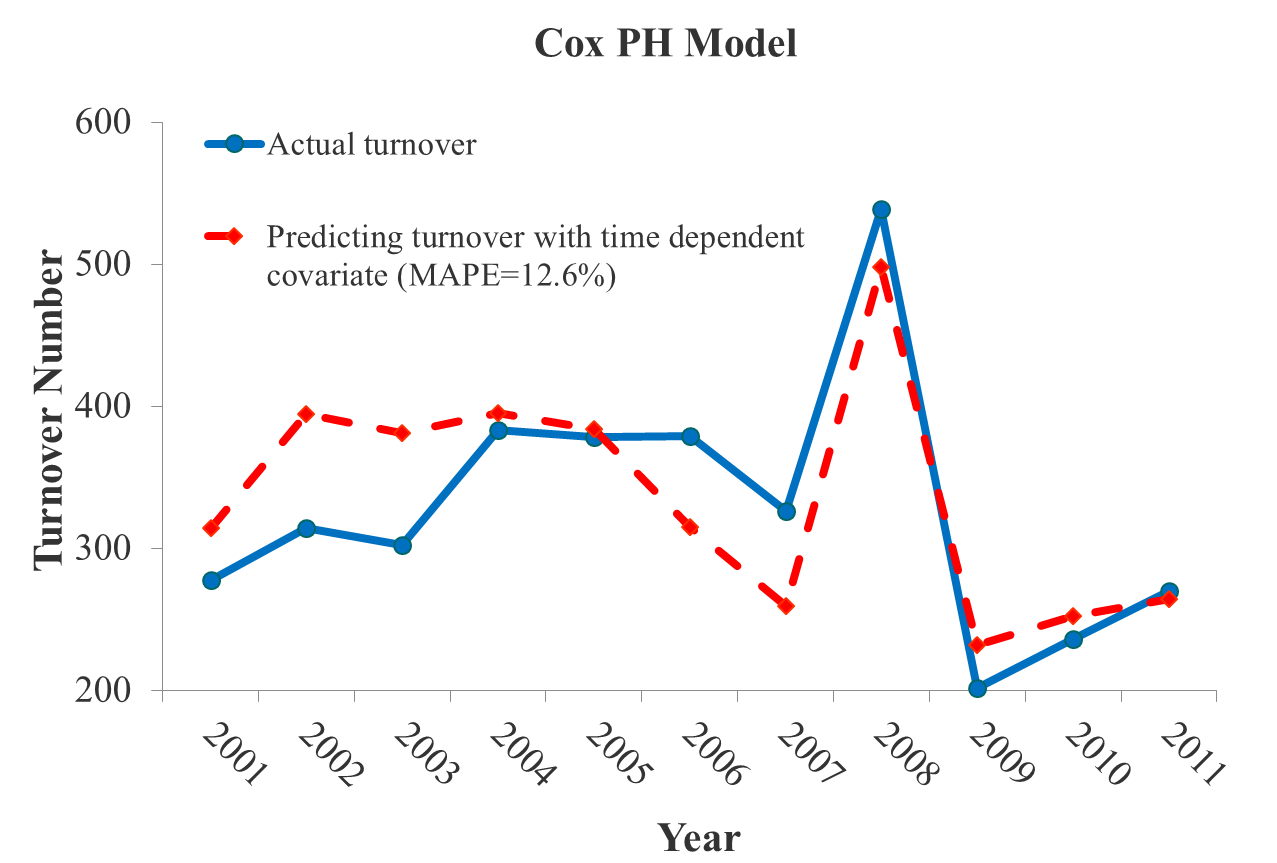
\includegraphics[width=5.5in]{Fig9.png}
	\caption{Actual vs. predicted turnover number for Cox PH model}
	\label{fig:9}
\end{figure}


%%%%%%%%%%%%%%%%%%%%%%%%%%%%
%%%%%%%%%%%%%%%%%%%%%%%%%%%%
%%%%%%%%%%%%%%%%%%%%%%%%%%%%
\subsection{Right censoring simulation result}
The right censoring simulation result shows Cox PH model coefficient estimate, baseline parameter estimates for Weibull distribution, and $-$log likelihood value for models with no censoring, 25\%, 50\%, and 75\% censoring proportion as shown in Table \ref{table:rightcensor}. The events in the second column of the table indicate total failure events in the dataset without including censoring, which is $events=\sum_{i=0}^{4000}{\delta_i}$ where $\delta$ is censor variable. The coefficients of age for all four models are all close to 0.025, but it is over estimates (0.026) when high proportion of censoring (75\%) in the dataset. The overestimation is also shown by the estimates of shape parameter: the estimated value (1.539) for model with 75\% censoring is greater than $\alpha=1.5$. It underestimates the shape parameters when the censoring proportion is 25\% and 50\%, respectively. The most close estimation of shape is when there is no censoring in the data. The $-$log likelihood values decrease from low percentage censoring to high percentage censoring. Because the scale parameter is generated by the formula, there is no actual value of scale parameter to compare. However, compared to the estimated value from no censoring (2.668), the model overestimates with 25\% censoring (2.779), get close with 50\% censoring (2.675) and underestimates with 75\% censoring (1.539). The estimates decrease when the percentage of censoring increases. Overall, the estimates are close to actual simulated value when the censoring proportion is close to 50\%. However, it over- or under-estimates the coefficients when the censoring proportion is 75\%. The phenomenon is also verified by plotting the actual and predicted failure number in the figure \ref{fig:7}.  The red line is the actual failure number simulated by Weibull distribution. The dark blue line is the predicted failure number for the model with 75\% censoring which is higher than all the other three lines for predicted failure number before time 3.75 and overlaid with the other three lines after 3.75. The gap between this line and the others three lines reaches the largest value around time 1. The other three lines represent the predicted failure number from the model with no censor, 25\% censoring, and 50\% censoring, respectively. They are too close to be distinguished in the figure. Therefore, the right censoring simulation shows that the Cox PH model performs well and the estimates are close to the actual values when the censoring proportion is close to 50\%, and it deteriorates when the censoring proportion is 75\%, causing the overestimation of the total failure number.
% Table generated by Excel2LaTeX from sheet 'Sheet2'
% Table generated by Excel2LaTeX from sheet 'Sheet1'
\begin{table}[htbp]
	\renewcommand{\arraystretch}{1.5}
	\small
	\centering
	\caption{Right censoring simulation statistics}
	\begin{tabular}{ccrrrc}
		\hline
		\multirow{2}[2]{*}{Models} & \multirow{2}[2]{*}{Events} & \multicolumn{3}{c}{Variable estimate} & \multirow{2}[2]{*}{$-$ loglikelihood} \\ \cline{3-5}
		
		&       & Age   & Scale & Shape &  \\\hline
		No Censor & 4000  & \multicolumn{1}{c}{0.024} & \multicolumn{1}{c}{2.668} & \multicolumn{1}{c}{1.494} & 4127.4 \\
		25\% Censored & 3000  & \multicolumn{1}{c}{0.025} & \multicolumn{1}{c}{2.779} & \multicolumn{1}{c}{1.480} & 3446.3 \\
		50\% Censored & 1999  & \multicolumn{1}{c}{0.024} & \multicolumn{1}{c}{2.675} & \multicolumn{1}{c}{1.487} & 2574.1 \\
		75\% Censored & 1000  & \multicolumn{1}{c}{0.026} & \multicolumn{1}{c}{2.643} & \multicolumn{1}{c}{1.539} & 1486.9 \\
		\hline
	\end{tabular}%
	\label{table:rightcensor}%
\end{table}%
\begin{landscape}
\begin{figure}[htbp]
	\centering
	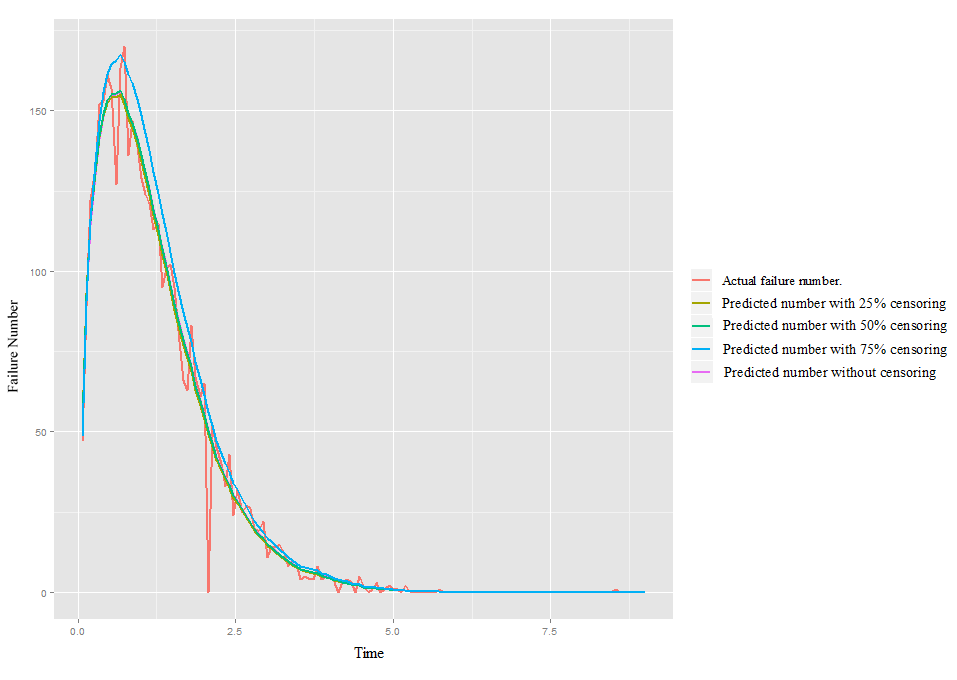
\includegraphics[width=9in]{Fig7}
	\caption{Actual vs. predicted failure number with various censoring}
	\label{fig:7}
\end{figure}
\end{landscape}
% % % % % % % % % % % % % % % % % % % % % % % % %
% % % %Left truncation result % % % % % % % % % % 
% % % % % % % % % % % % % % % % % % % % % % % % %
\subsection{Left truncation simulation results}
The left truncation bias simulation statistics for testing Cox PH model function shows coefficient estimate for age, baseline parameter estimates for scale and shape by Weibull distribution, $-$log likelihood value, and total predicted failure number for models with no left truncation, 25\%, 50\%, and 75\% left truncation proportion as shown in Table \ref{tab:lefttruncation}. The coefficients of age for all four models are all close to 0.025, even when high proportion of left truncation (75\%) in the dataset. However, the scale and shape parameter are over estimated, when the left truncation proportion is high: the estimated values for scale are 2.656, 2.620, 2.664, and 2.748 for no left truncation, 25\%, 50\%, and 75\%, respectively. The estimated values for shape are 1.483, 1.501, 1.504, and 1.539 for no left truncation, 25\%, 50\%, and 75\%, respectively. The estimation of the scale and shape for Weibull  distribution is close to simulation value when the left truncation portion is 25\% and 50\%. The model overestimates the parameters when left truncation proportion is 75\%, which is greater than $\alpha=1.5$. The last column is the summation of predicted failure number at each time point. They are close to actual failure number (4005, 2992) when left truncation proportion is 0\% and 25\%, respectively. When left truncation reaches to 50\% and 75\%, the failure number are around 50 more than the actual (2051 and 1059). However, the predicted failure number is smoothed and close to the actual one as shown in the figure \ref{fig:lefttruncation}. It is overestimates at the beginning of the time line when left truncation proportion is 50\% and 75\% as shown in figure \ref{fig:left50} and \ref{fig:left75}, where the dash lines are both higher than the solid lines at the beginning. 
Therefore, the left truncation simulation test shows that the Cox PH model performs well when the censoring proportion is less than 50\%, and it deteriorates when the truncation proportion goes high causing the overestimation of the total failure number.
\begin{table}[h!]
	\renewcommand{\arraystretch}{1.5}
	\small
	\centering
	\caption{Left truncation simulation statistics}
	\begin{tabular}{ccccccc}
		\hline
		\multirow{2}[4]{*}{Model} & \multirow{2}[4]{*}{Events} & \multicolumn{3}{c}{Variable Estimates} & \multirow{2}{3cm}{$-$ log.Likelihood} & \multirow{2}{3cm}{Predicted Total Failure No.}  \\
		\cline{3-5} % \cline{i-j} partial horizontal line beginning in column i and ending in column j		
				&       & Age   & Scale & Shape &  &\\				
		\hline
		No left Truncation & 4000  & 0.024 & 2.656 & 1.483 & 4167.8  &4005\\
		25\%  left Truncation & 3000  & 0.023 & 2.620  & 1.501 & 3041.2 & 2992\\
		50\%  left Truncation & 2000  & 0.023 & 2.664 & 1.504 & 1990.8 & 2051\\
		75\%  left Truncation & 1000  & 0.025 & 2.748 & 1.539 & 885.55 &2059\\
		\hline
		\end{tabular}%
	\label{tab:lefttruncation}%
\end{table}%
%negative loglikelihood value can be dropped. does not make sense.

\begin{figure}[h!]
	\centering
	\subfloat[No left truncation]{\label{fig:leftno}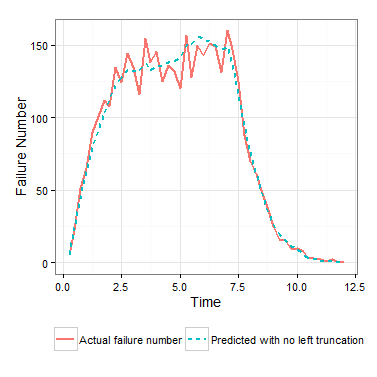
\includegraphics[width=2.75in]{notruncation.png}}
    \quad
	\subfloat[25\% left truncation]{\label{fig:left25}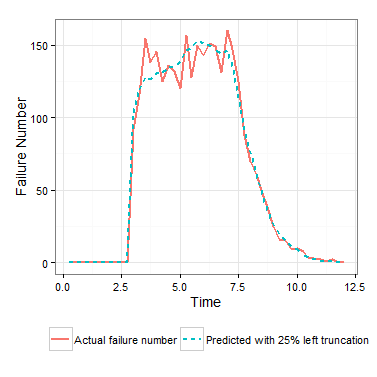
\includegraphics[width=2.75in]{25color.png}}
	\quad
	\subfloat[50\% left truncation]{\label{fig:left50}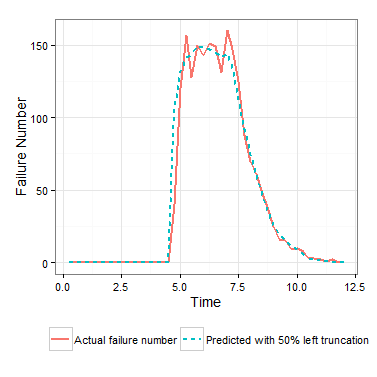
\includegraphics[width=2.75in]{50color.png}}
	\quad
	\subfloat[75\% left truncation]{\label{fig:left75}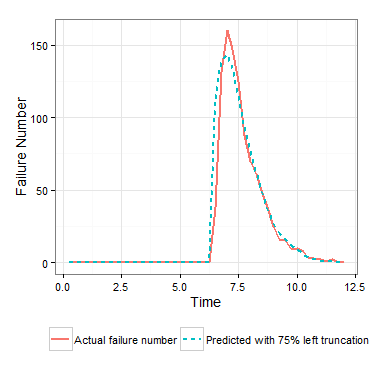
\includegraphics[width=2.75in]{75color.png}}
	\caption{Left truncation simulation results: actual vs. predicted failure number}
	\label{fig:lefttruncation}
\end{figure}
\subsection{Variable Selection}
The payroll is dropped from the variable list, because it is highly associated with Cocs as shown in table \ref{tab: freq1}. C and R are hourly payroll. E, M, and S are monthly payroll. G and T are weekly payroll. Only L and P have two levels of payroll, but L is mainly hourly payroll, and P is mainly monthly payroll. Their small parts are not reach 1\% of total employee number. Thus, the payroll is dropped from variable list.          
\begin{table}[htbp]
	\centering
	\small
	\renewcommand{\arraystretch}{1.5}
	\caption{ Table of Payroll by Cocs in percentage }
	\begin{tabular}{llllllllllll}
		\hline
		\multirow{2}[4]{*}{Payroll} & \multicolumn{10}{c}{Cocs} \\ \cline{2-11}
		
	
		& C     & E     & G     & L     & M     & P     & R     & S     & T     & Total \\ \hline
		H     & 14.27 & 0     & 0     & 8.78  & 0     & 0     & 6.75  & 0     & 0     & 29.79 \\
		M     & 0     & 16.45 & 0     & 0     & 16.01 & 20.66 & 0     & 2.38  & 0     & 55.50 \\
		W     & 0     & 0     & 6.27  & 0.35  & 0     & 0.01  & 0     & 0     & 8.08  & 14.71 \\
		Total & 14.27 & 16.45 & 6.27  & 9.12  & 16.01 & 20.67 & 6.75  & 2.38  & 8.08  & 100 \\
		\hline
	\end{tabular}%
	\label{tab: freq1}%
\end{table}%



    \chapter{Employee Voluntary Turnover Determinants Analysis and Forecasting for R\&D Departments} \label{ch:4}
\section{Introduction}
Researchers and human resource managers have focused on employee turnover for decades because it has negatively affects organizations' performance \citep{shaw2011}. Employee retention is one of the main challenges in organizations, especially for those with a long lead time to hire a new employee. In this study, besides the hiring and training time, the background security check takes a long time ($>6$ months) when filling positions. Our study's subjects were 731 terminated employees in four research and development departments across more than a ten-year study window. This study focuses on employee voluntary turnover, i.e., employees who voluntarily quit their job. Among the reasons for termination, voluntary turnover is one of the major ones, accounting for 26\%. Compared to retirement and layoff, voluntary turnover is harder for companies to control. Because voluntary turnover is expensive for companies \citep{selden2000}, they do not want their employees to voluntarily leave \citep{allen2010}. Therefore, this study's objective is to examine what determines voluntary turnover for R\&D department employees and to forecast employee tenure, thus assisting in hiring decisions. 

\section{Literature Review}
Employee turnover represnets a major loss of intellectual property to an organization. The total cost associated with employee turnover is estimated to range from 100-300\% of a departing employee's annual salary \citep{Moody2000}. Both private firms and governmental organzations spend billions of dollars every year to manage employee turnover \citep{leonard2001}. Furthermore, employee turnover can significantly reduce the production system's reliability \citep{ahmad2014, sawhney2010}. For organizations to execute their tasks efficiently and effectively with the highest quality, they must ensure that the right people are available at the right places and at the right times \citep{khoong1996}. 
Many researchers have attempted to identify turnover factors to prevent and reduce turnover. \citet{bluedorn1982} reported that turnover is related to an individual's, routine, age, length of service, and perception of environmental opportunities. \citet{balfour1993} suggested that caseworkers with more education, less experience, and less at stake in an organization are more likely to turnover. According to \citet{griffeth2000}, pay and pay-related variables modestly affect turnover. They also examined the relationship among pay, a person's performance, and turnover. They concluded that when high performers are inadequately rewarded, they quit. In our dataset, company job titles are highly and positively correlated with employees' salaries, sensitive information that cannot be released. We can hypothesize the following:

\textbf{Hypothesis 1: The company job title is a significant predictor of voluntary turnover.}

Besides job titles, we think employees' college majors are also a factor causing variation of employees' salaries. Thus, we hypothesize the following:

\textbf{Hypothesis 2: The college major (branch of study) is a predictor of voluntary turnover. }

\citet{griffeth2000} study shows that employees' demographic characteristics such as gender and education level are also highly correlated to employee turnover. They also found that men are less likely to turnover than women. Thus, we hypothesize the following:

\textbf{Hypothesis 3: Employee education level is correlated with employee voluntary turnover.}


\textbf{Hypothesis 4: Female employees are more likely to voluntary turnover than male employees.}

Many researchers have examined the relationship between employees' age and turnover. Younger employees are more likely to move from one job to another \citep{burke1994}, particularly those less than 35 years old \citep{RN45}. Thus, we hypothesize the following:

\textbf{Hypothesis 5: Age is an important factor in employee voluntary turnover.}

Employees are more likely to quit during the first five years before they have a strong commitment to the organization. \citet{bluedorn1982} found that turnover is related to length of service. Thus, we hypothesize the following:

\textbf{Hypothesis 6: Length of service is an important factor in employee voluntary turnover.}

Furthermore, some races may react differently to other races. For example, \citet{RN42} found that employee turnover is significantly related to race. Ethnic minorities' language and accent barriers may cause social differences with the ethnic majority. Thus, we hypothesize the following:

\textbf{Hypothesis 7: Ethnicity is related to employee voluntary turnover.}

Many researchers have used logistic regression to build models and to identify turnover's attributes. For example, \citet{balfour1993} applied logistic regression to build an employee turnover model. \citet{wright1998} used correlation and logistic regression to examine whether emotional exhaustion is a predictor of turnover. \citet{morrow1999} applied logistic regression to determine whether employees' absence and performance record can be employee-turnover indicators. \citet{nagadevara2008} applied several statistical methods including logistic regression to predict employee turnover.
To predict employee turnover behavior, many other statistical techniques (such as regression, neural network (NN), and data mining) have also been used. For example, \citet{ng1991} used a proportional hazards regression (PHR) to develop a turnover prediction model. \citet{RN6} developed a turnover prediction model for accountants in a Singapore organization. \citet{RN8} used multiple regression to explore turnover intention. \citet{RN10} combined Taguchi's method and Nearest Neighbor Classification Rules to select feature subsets and analyze factors to find the best predictor of employer turnover. \citet{alao2013} used a decision tree to classify employees based on various types of attrition using employees' records. However, all these modeling methods have attempted to forecast employees' turnover behaviors rather than providing a forecast model or rules that forecast employee tenure and that also assist in hiring employees who are less likely to voluntarily quit. 

This chapter has five parts. Part one is the introduction including the objective and literature review. Part two provides a synopsis of tools for data preparation and discusses forecasting methods. Part three presents results. Part four discusses the results. Part five is the conclusion. 
\section{Methodology}
\subsection{Data and preparation}
In 2011 a large U.S. organization provided the human resource data for this study. The dataset contained 731 observations of terminated employee records from October 2000 to June 2011, including metrics such as ID, division (department), job title, termination reason, last hired date, termination date, years of service (YCS), gender, race, age at hiring, age at termination, highest education degree, and branch of study. 
In addition, two variables were created from the dataset for analysis. One variable was major, including 15 levels. The first three letters of the branch of study are used for identification; for example, Eng refers to engineering, and Che refers to chemistry. The other was a binary target variable Y for logistic regression. Y is equal to 1 if an employee voluntarily quits; otherwise, y is equal to 0 if an employee leaves the organization for other reasons.
\subsection{Logistic regression}
The hypotheses were tested using logistic regression to identify voluntary turnover's significant predictors. Logistic regression, or logit regression, is a popular model for binary data \citep{RN57}. It is used to predict a binary response from a binary predictor, to predict a categorical variable's outcome based on one or more predictor variables, and to estimate a qualitative response model's parameters. Unlike linear regression, logistic regression can handle both categorical and numeric variables. The logistic regression is expressed in Equation \ref{eq:logit}
\begin{equation}
logit[\pi(x)]=log(\frac{\pi(x)} {1-\pi(x)})= \alpha+\beta x  
\label{eq:logit}            
\end{equation}
where $x$ represents the explanatory variables; $\pi(x)$ denotes the target variable's probability at value $x$; $\frac{\pi(x)} {1-\pi(x)}$ is the odds of $x$; and $\alpha$, $\beta$ are the estimated coefficients. All the predictors were tested using 0.05 as a p value criteria. The other variables, such as department, were also included in the model to eliminate the other variables' variance. Three statistics criteria were used to evaluate the logistic regression model: Akaike's information (AIC), Schwartz's Bayesian criterion (SBC), and the Hosmer-Lemeshow Goodness of Fit Test. AIC and SBC are both information criteria using likelihood value. Usually, the best model comes with the lowest AIC or SBC values. The Hosmer-Lemeshow test is a chi-square test to determine whether the logistic regression model is correctly specified \citep{hosmer2004}. The high p-value ($P>0.05$) indicates that this model passes the test. 
\subsection{Decision tree}
A decision tree, also called a classification tree, is one method of classification via an intermediate tree-like structure in data mining \citep{hand2001}. A decision tree's purpose is to develop a classification rule from the data based on attributes, or explanatory variables. Similar to logistic regression, a decision tree can handle categorical or numeric variables. Creating a decision tree involves splitting the significant variable until only one unique classification is on each branch of the tree. The decision tree was used for data compression and prediction. 
In this study, YCS were used as a target variable generating a classification rule for managers and human resource departments to forecast how many years an employee will work in the organization. It also provides managers a tool for making accurate hiring decisions. The turnover dataset was divided into two parts: training (60\%) used to build a decision tree and validation (40\%) used to validate the model performance. The decision tree model was built using AIC values as model selection criteria. The decision tree was analyzed using SAS Enterprise Miner 7. 
\section{Results}
\subsection{Hypothesis test results}

All variables proposed in the hypothesis were tested with other control variables using the logistic regression model. The parameter estimations are shown in Table \ref{tab:logitpar}. The variables included Div (division), jobtitle (job title), race, gender, degree (highest education degree), major (branch of study), age (age at termination), and YCS (years of company service). Five variables were statistically significant ($P<0.05$) in the logistic regression model: jobtitle, gender, race, age and YCS. This finding indicates that employees voluntarily quitting the organization are statistically affected by their company job title, gender, race, age, and years of company service.

\begin{table}[http]
	\centering
	\caption{Logistic Regression Parameter Estimates}
	\label{tab:logitpar}
	\begin{tabular}{llll}
		\toprule
		Effect           & DF & Wald$\chi^2$ & $Pr>\chi^2 $ \\
		\midrule
		Jobtitle         & 14 & 37.21                    & \textless.01                     \\
		Division         & 3  & 4.07                     & 0.25                               \\
		Gender           & 1  & 10.72                    &  .001                              \\
		Degree           & 5  & 2.25                     & 0.81                               \\
		Major            & 14 & 9.75                     & 0.78                               \\
		Race             & 4  & 30.56                    & \textless.01                      \\
		Age              & 1  & 38.81                    & \textless.01                      \\
		Years of Service & 1  & 45.62                    & \textless.01     \\
		\bottomrule                
	\end{tabular}
\end{table}
The results of the hypotheses tests are discussed below.

\textbf{Hypothesis 1: The company job title is a significant predictor of voluntary turnover.}

The company job title is a pivotal factor in voluntary turnover since it is highly associated with employee salary ($\chi^2=37.2, df=14, P<0.05$). We have no evidence to reject the null hypothesis. Compared to the reference group (Managers), four job title groups are statistically significantly different than the manager group. This company's job titles are Administrator 1, Administrator 2, Administrator 3, Staff Level 1, and Technician; their coefficient estimates are -6.7 -2.9, -3.6, -1.8 and -3.0, respectively. These results show that compared with managers, employees in these positions are less likely to quit: Administrator 1 has 99.9\% (1-exp(-6.7)) less odds; Administrator 2 has 94.5\% less odds; Administrator 3 has 97.3\% less odds; Staff 1 has 83.4\% less odds; and Technician has 95\% less odds. The other job titles are not statistically significant, indicating they have the same turnover odds as managers.

\textbf{Hypothesis 2: The college major (branch of study) is a predictor of voluntary turnover. }

According to Table 1, employees' major has 9.7 of Wald $\chi^2$ with 14 degrees of freedom, and P value is 0.78. We have evidence to reject the null hypothesis. Employees' college major (branch of study) does not significantly affect employee turnover behaviors in R\&D departments. 

\textbf{Hypothesis 3: Employee education level is correlated with employee voluntary turnover.}

In this study, an education degree is not significantly correlated with employee voluntary turnover ($\chi^2=2.25, df=5, P=0.81$). We have evidence to reject the null hypothesis, thus showing that employees with a higher education degree have voluntary turnover behavior similar to those without a higher education degree. 

\textbf{Hypothesis 4: Female employees are more likely to voluntary turnover than male employees. }

We do not have evidence to reject the null hypothesis. Gender is also significant ($\chi^2=10.7, df=1, P<0.05$), indicating that female and male employees have different voluntary quit behaviors, as the parameter estimation for female is 1.29. Also, the odds of female voluntary turnover are 3.6 times that of male employees, indicating female employees are more likely to voluntarily quit. 

\textbf{Hypothesis 5: Age is an important factor in employee voluntary turnover.}

We do not have evidence to reject this null hypothesis. Employees' age significantly affects voluntary turnover ($\chi^2=38.8, df=1, P<0.05$). The coefficient estimate is -0.13 and the odds ratio is 0.87, indicating that the turnover odds decrease 13\% when an employee's age increases one year older. As a result, younger employees tend to be more likely to quit than older employees.    

\textbf{Hypothesis 6: Length of service is an important factor in employee voluntary turnover.}

We do not have evidence to reject this null hypothesis. Employees' years of service significantly affect voluntary turnover ($\chi^2=45.6, df=1, P<0.05$). The coefficient estimate is -0.15 and the odds ratio is 0.86, indicating that the turnover odds decrease 14\% with each additional year of service. Thus, employees with fewer years of service tend to be more likely to quit.        

\textbf{Hypothesis 7: Ethnicity is related to employee voluntary turnover.}

We do not have evidence to reject this null hypothesis. Ethnicity has a statistical impact on employee voluntary turnover behavior ($\chi^2=30.6, df=4, P<0.05$). Asian, Black or African American, and Hispanic/Latino are significantly different statistically from white employees, the reference group, in terms of turnover because these three groups have negative coefficient estimates. Black or African American employees have the lowest coefficient estimates (-3.7) and odds ratio (0.024=exp(-3.7)). Asian and Hispanic/Latino employees have -1.3 and -1.5 of coefficients and 0.27 and 0.22 of odds ratio, respectively. These three groups have lower turnover probability than white employees. However, Native American employees are not significantly different statistically from white employees ($P > 0.05$), showing that Native American employees have the same turnover probability as white employees. 
\subsection{Decision tree analysis results}

This study's decision tree model is a five-level depth tree with 17 nodes and has the lowest AIC value. Four variables are statistically significant in the model: \textit{ageh} (age at hire), \textit{jobtitle} (job title), \textit{div} (division), and \textit{race}. The most important variable is \textit{ageh} located in the decision tree's first, third, and fourth nodes, indicating that an employee's YCS is mainly determined by age when hired. Two other variables, job title and division, also significantly affect an employee's YCS. Based on the model, DIV1 is significantly different from the other three departments (DIV 2, DIV3, and DIV4). The employees with the following job titles are significantly different from those with other job titles: Staff 2, Staff Member 1, Administrator 2, or Administrator 1. Compared to other ethnicities, white employees have more YCS if they are younger than 28 when hired. The decision tree's rules are the following:
\begin{itemize}
	\item if $ageh \ge 42.25 $ and $div=$DIV1, then  $E(YCS)=11.9$;
	\item if $ageh \ge  42.25$ and $div\neq$ ES1, then $E(YCS)=5.6$;
	\item if $21.35 \le ageh < 42.25$, $job title =$ (Staff 2, Staff Member 1, Administrator 2, or Administrator 1), and $div= $DIV1, then $E(YCS)=22.9$;
	\item if $ageh < 42.25$, $job title =$ (Staff 2, Staff Member 1, Administrator 2, or Administrator 1), $div= $DIV1, and $ageh < 21.35$, then $E(YCS)=4.9$;
	\item if $ageh < 42.25$, $job title =$ (Staff 2, Staff Member 1, Administrator 2, or Administrator 1), and $div\neq$ DIV1, then $E(YCS)=2.5$;
	\item if $27.95 \le ageh < 42.25$, $job title \neq $ (Staff 2, Staff Member 1, Administrator 2, or Administrator 1), and $div=$ DIV2, DIV3, or DIV4 then $E(YCS)=12.1$;
	\item if $27.95 \le ageh < 42.25$, $job title \neq $ (Staff 2, Staff Member 1, Administrator 2, or Administrator 1), and $div neq$ DIV2, DIV3, or DIV4 then $E(YCS)=22.8$;
	\item if $ ageh < 42.25 $, $job title \neq $ (Staff 2, Staff Member 1, Administrator 2, or Administrator 1), $ageh<27.95$ , and $race=$ white or white/non-Hispanic origin, then $E(YCS)=29.8$;
	\item if $ ageh < 42.25 $, $job title \neq $ (Staff 2, Staff Member 1, Administrator 2, or Administrator 1), $ageh<27.95$ , and $racegroup\neq$ white or white/non-Hispanic origin, then $E(YCS)=17.8$;
	
\end{itemize}
where, E(YCS) denotes expected or average YCS. The predicted YCS's range is from 2.5 to 29.8 years. The model's performance is validated by predicting E(YCS) in the validation dataset. As shown in Figure \ref{fig:decsiontree}, the predicted values are close to the actual values in each leaf, indicating the decision tree model has strong forecasting ability. After the decision rule is determined, predicting YCS for a new employee is easily calculated by following the rules. This ease of calculation is one of the decision tree method's advantages. 
\begin{figure}
	\centering
	\includegraphics{decisiontree.png}
	\caption{Actual vs. Predicted E(YCS) for Validation Dataset}
	\label{fig:decsiontree}
\end{figure}
\section{Discussion}
This study's purposes were to investigate factors contributing to R\&D employee voluntary turnover and to support employee hiring and retention strategies. The logistic regression's results show that job title, gender, ethnicity, age, and years of service are significant predictors of employee turnover. However, an employee's division, education level, and major are not associated with employee turnover. 

Although we found that employee job title is a significant predictor of employee turnover, the comparison results show that employees with lower salaries are more likely to stay. This finding is different from the previous study. Compared to the other staff levels, level 1 staff are also more likely to stay because they do not have much work experience. Also, their average salary is 20\% higher than the job market's average. On the other hand, the other staff levels have the same probability to quit as the reference group (managers). According to \citet{RN37} study, when employees find no opportunities for advancement within the system, they will not remain in the work situation. The promotion competition is intense among R\&D staff members with the same education degree and experience. However, they easily find higher paying positions in other companies or become members of faculty or research staff in organizations when they have several years of work experience. Therefore, R\&D staff are more likely to quit when they are not in staff level 1.  

Furthermore, female employees are more likely to quit than male employees. According to the work/family life-balance theory \citep{RN38}, as economic pressure increases, an employee may have to do the work of more than one person. Especially when an organization downsizes or restructures, the same amount of work has to be done by fewer employees. Thus, employees spend more time on their work life and have less time for their personal life \citep{smith2009}. Female employees serve a more important role in the family than male employees. Forced to make a choice between family and work, female employees are more likely to quit. 

Many studies have proved that age has a negative relationship with turnover \citep{rhodes1983}. Researchers believe younger workers leave for two main reasons: lack of training opportunities and lack of mentors in the workplace \citep{paul2012}. Although many managers are promoted because of their strong capability and achievement, they are not nescesarily good coaches or team leaders and are unable to help employees improve their performance \citep{smith2009}. Furthermore, R\&D employees work more independently than employees in other departments. For example, sometimes one employee is responsible for one project or part of a project. Compared to experienced staff, younger staff feel frustrated and stressed when they meet difficulties or barriers and cannot receive adequate advice. As a result, younger employees are more likely to voluntarily leave.  

The number of years an employee has worked in the organization is another significant factor in turnover. Many studies have found that length of service is highly related to organization commitment \citep{Jena2015, Kelarijani2014, Popoola2006}. The longer the employee works, the more that employee feels attached to and involved in the organization. As a result, employees with longer length of service are more likely to stay. On the other hand, employees with few years of service have not formed a strong commitment to the organization. Thus, they tend to switch to a new job to increase their work experience, receive higher pay, or be in a higher position.

Ethnicity is another significant factor affecting employee turnover. According to our analysis, Black or African American employees have the lowest probabilities of quitting compared to the other ethnic groups. Asian and Hispanic employees are also less likely to quit than the white employees in the study. However, Native American/Alaskan employees have the same turnover probability as white employees.   

Employee turnover does not correlate with majors as shown in Table 1. Although some majors like computer science or engineering have more job openings, they do not have a higher turnover probability in R\&D departments because employees have 20\% higher salaries than the job market's average levels, according to our study. 

Education degree is not a significant factor in voluntary turnover. Most employees (80\%) in the four R\&D departments are highly educated with at least a bachelor's degree. However, technicians and administrators are more likely to have a high school or an associate's degree. As discussed above, they are all less likely to quit. Therefore, determining which employees with which degree are more likely to quit is difficult.
Employee division in this study is not significant ($\chi^2=4.7, df=3, P > 0.05$). The results indicate that employees have the same turnover probability among the four divisions, which have similar structures and cultures. 
 
The decision tree model predicts the average employee's working years in the R\&D department under all types of employee turnover. The significant variables$-$age when an employee was hired, job title, division, and ethnicity$-$are easily obtainable. Based on the decision rules, managers can quickly determine whether an interviewee will have a long or short tenure. Based on the rules shown in section 4.2, a new employee's years of service can be predicted. If a new employee is applied to rules (2), (4), and (5), that employee's predicted YCS will be fewer than 10 years. If a new employee is applied to rules (1), (6), and (9), the predicted YCS will be 10 to 20 years. If a new employee is applied to rules (3), (7), and (8), the predicted YCS will be above 20 years.
\section{Conclusions and Recommendations}
In this study, employee turnover's significant attributes and classification rules were identified based on employee records from four R\&D departments. Seven variables in the hypothesis were tested in the logistic regression model to find the variables' significance. This logistic regression determined the probability of an employee's voluntary turnover and identified four significant factors affecting voluntary turnover: job title, gender, ethnicity, age, and years of service. These results can assist managers and human resource departments in developing employee-retention strategies to reduce R\&D departments' voluntary turnover rate.  
 
The decision tree generated nine rules to predict the average length of YCS of an employee. The models' results showed that combining models was suitable for forecasting employee turnover. Applications of the models can be used with hiring strategies. For example, when the data and related variables are accessible, a decision tree can generate a decision rule, such as hiring or not hiring an applicant. Results from the decision tree indicated that the age of employees when hired was the most important variable. 

Several statistical software packages are available to conduct logistic regression and decision tree models, such as SAS, SPSS. If human resource departments have limited budgets, they can also use statistical software R, which is a free open source. These two models are created based on the termination dataset with limited variables. If more data and variables can be identified, the models can be further improved. 




    %%%%%%%%%%%%%%%%%%%%%%%%%%%%%%%%%%%%%%%%%%%%%%%%%%%%%%%%%%%%%%%%%%%%%%%%%%%%%%%%%%%%%%%%%%%%%%%%%%%%%
    % BIBLIOGRAPHY
    %%%%%%%%%%%%%%%%%%%%%%%%%%%%%%%%%%%%%%%%%%%%%%%%%%%%%%%%%%%%%%%%%%%%%%%%%%%%%%%%%%%%%%%%%%%%%%%%%%%%%
    \makeBibliographyPage % make the bibliography title page - can be edited in ut-thesis-template.tex
    \bibliographystyle{apalike} % bibliography style - recommend using apalike-doi as it hyperlinks DOIs
    \bibliography{references/references-dissertation} % references.bib included in the references directory
    %%%%%%%%%%%%%%%%%%%%%%%%%%%%%%%%%%%%%%%%%%%%%%%%%%%%%%%%%%%%%%%%%%%%%%%%%%%%%%%%%%%%%%%%%%%%%%%%%%%%%
    % APPENDIX - OPTIONAL - COMMENT IF NOT NEEDED
    %%%%%%%%%%%%%%%%%%%%%%%%%%%%%%%%%%%%%%%%%%%%%%%%%%%%%%%%%%%%%%%%%%%%%%%%%%%%%%%%%%%%%%%%%%%%%%%%%%%%%
    \makeAppendixPage   % make the appendix title page - can be edited in ut-thesis-template.tex
    \appendix
    \include{back-matter/appendix-1}
    %%%%%%%%%%%%%%%%%%%%%%%%%%%%%%%%%%%%%%%%%%%%%%%%%%%%%%%%%%%%%%%%%%%%%%%%%%%%%%%%%%%%%%%%%%%%%%%%%%%%%
    % A VITA IS REQUIRED
    %%%%%%%%%%%%%%%%%%%%%%%%%%%%%%%%%%%%%%%%%%%%%%%%%%%%%%%%%%%%%%%%%%%%%%%%%%%%%%%%%%%%%%%%%%%%%%%%%%%%%
    \addToTOC{Vita}
    \include{back-matter/vita}
\end{document}
